\chapter{Protocols for 2 qubit gates}
\label{chap:2_qubit_gates}

To execute experiments and induce the emission of entangled photons into the waveguide, conducting both single- and two-qubit gates on our device is essential.
As previously explained in the preceding chapter, conducting single-qubit gates on the emitter qubits is not viable due to their short lifespans.
This limitation also influences the type of two-qubit gate feasible between a storage and an emitter qubit.
For instance, we are unable to perform a controlled-phase gate, or CZ gate, between a storage and an emitter.

In this chapter, we will discuss the types of two-qubit gates that we can perform between storage-storage and storage-emitter qubits.
The gates we are able or unable to perform is the main limiting factor affecting the number of entangled photonic states we can create with our device.

\section{Storage-Emitter operations}
\label{sec:S-E}

In \cref{fig:level_S-E} we illustrate the level diagram for a storage-emitter (S-E) system.
\begin{figure}[h]
    \centering
    

\tikzset{every picture/.style={line width=0.75pt}} %set default line width to 0.75pt        

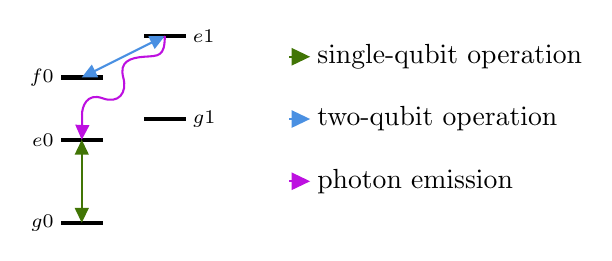
\begin{tikzpicture}[x=0.75pt,y=0.75pt,yscale=-1,xscale=1]
%uncomment if require: \path (0,300); %set diagram left start at 0, and has height of 300

%Straight Lines [id:da9036150792074441] 
\draw [line width=1.5]    (100,100) -- (120,100) ;
%Straight Lines [id:da3892496668455091] 
\draw [line width=1.5]    (140,80) -- (160,80) ;
%Straight Lines [id:da8780144362496497] 
\draw [line width=1.5]    (100,130) -- (120,130) ;
%Straight Lines [id:da9845944648914766] 
\draw [line width=1.5]    (100,170) -- (120,170) ;
%Straight Lines [id:da40423833166537637] 
\draw [line width=1.5]    (140,120) -- (160,120) ;
%Straight Lines [id:da9138884186505395] 
\draw [color={rgb, 255:red, 65; green, 117; blue, 5 }  ,draw opacity=1 ]   (110,133) -- (110,167) ;
\draw [shift={(110,170)}, rotate = 270] [fill={rgb, 255:red, 65; green, 117; blue, 5 }  ,fill opacity=1 ][line width=0.08]  [draw opacity=0] (7.14,-3.43) -- (0,0) -- (7.14,3.43) -- cycle    ;
\draw [shift={(110,130)}, rotate = 90] [fill={rgb, 255:red, 65; green, 117; blue, 5 }  ,fill opacity=1 ][line width=0.08]  [draw opacity=0] (7.14,-3.43) -- (0,0) -- (7.14,3.43) -- cycle    ;
%Straight Lines [id:da18399826038705747] 
\draw [color={rgb, 255:red, 74; green, 144; blue, 226 }  ,draw opacity=1 ]   (147.32,81.34) -- (112.68,98.66) ;
\draw [shift={(110,100)}, rotate = 333.43] [fill={rgb, 255:red, 74; green, 144; blue, 226 }  ,fill opacity=1 ][line width=0.08]  [draw opacity=0] (7.14,-3.43) -- (0,0) -- (7.14,3.43) -- cycle    ;
\draw [shift={(150,80)}, rotate = 153.43] [fill={rgb, 255:red, 74; green, 144; blue, 226 }  ,fill opacity=1 ][line width=0.08]  [draw opacity=0] (7.14,-3.43) -- (0,0) -- (7.14,3.43) -- cycle    ;
%Straight Lines [id:da14000382288661184] 
\draw [color={rgb, 255:red, 65; green, 117; blue, 5 }  ,draw opacity=1 ]   (210,90) -- (217,90) ;
\draw [shift={(220,90)}, rotate = 180] [fill={rgb, 255:red, 65; green, 117; blue, 5 }  ,fill opacity=1 ][line width=0.08]  [draw opacity=0] (8.93,-4.29) -- (0,0) -- (8.93,4.29) -- cycle    ;
%Straight Lines [id:da9331304771806838] 
\draw [color={rgb, 255:red, 74; green, 144; blue, 226 }  ,draw opacity=1 ]   (210,120) -- (217,120) ;
\draw [shift={(220,120)}, rotate = 180] [fill={rgb, 255:red, 74; green, 144; blue, 226 }  ,fill opacity=1 ][line width=0.08]  [draw opacity=0] (8.93,-4.29) -- (0,0) -- (8.93,4.29) -- cycle    ;
%Curve Lines [id:da6855478455179863] 
\draw [color={rgb, 255:red, 189; green, 16; blue, 224 }  ,draw opacity=1 ]   (150,80) .. controls (150,90.17) and (147,89.5) .. (140,90) .. controls (133,90.5) and (128,92.5) .. (130,100) .. controls (132,107.5) and (127.67,112.83) .. (120,110) .. controls (112.33,107.17) and (110.08,114.29) .. (110.13,117.88) .. controls (110.16,120.62) and (110.16,123.77) .. (110.09,127.01) ;
\draw [shift={(110,130)}, rotate = 272.25] [fill={rgb, 255:red, 189; green, 16; blue, 224 }  ,fill opacity=1 ][line width=0.08]  [draw opacity=0] (7.14,-3.43) -- (0,0) -- (7.14,3.43) -- cycle    ;
%Straight Lines [id:da22870453087792075] 
\draw [color={rgb, 255:red, 189; green, 16; blue, 224 }  ,draw opacity=1 ]   (210,150) -- (217,150) ;
\draw [shift={(220,150)}, rotate = 180] [fill={rgb, 255:red, 189; green, 16; blue, 224 }  ,fill opacity=1 ][line width=0.08]  [draw opacity=0] (8.93,-4.29) -- (0,0) -- (8.93,4.29) -- cycle    ;

% Text Node
\draw (98,100) node [anchor=east] [inner sep=0.75pt]  [font=\scriptsize]  {$f0$};
% Text Node
\draw (98,130) node [anchor=east] [inner sep=0.75pt]  [font=\scriptsize]  {$e0$};
% Text Node
\draw (98,170) node [anchor=east] [inner sep=0.75pt]  [font=\scriptsize]  {$g0$};
% Text Node
\draw (162,80) node [anchor=west] [inner sep=0.75pt]  [font=\scriptsize]  {$e1$};
% Text Node
\draw (162,120) node [anchor=west] [inner sep=0.75pt]  [font=\scriptsize]  {$g1$};
% Text Node
\draw (222,90) node [anchor=west] [inner sep=0.75pt]   [align=left] {single-qubit operation};
% Text Node
\draw (222,120) node [anchor=west] [inner sep=0.75pt]   [align=left] {two-qubit operation};
% Text Node
\draw (222,150) node [anchor=west] [inner sep=0.75pt]   [align=left] {photon emission};


\end{tikzpicture}
    \vspace{-1cm}
    \caption{Level diagram of storage-emitter interaction}
    \label{fig:level_S-E}
\end{figure}

We label the levels of the storage qubit with $\ket{g}, \ket{e}, \ket{f}$ and those of the emitter as $\ket{0}, \ket{1}$.
Due to the rapid emission of the emitter, the second excited level $\ket{2}$ is not relevant for our purposes.
In addition, we cannot run single-qubit gates on the emitter.
The only operations we can execute are single-qubit gates on the storage qubit and two-qubit gates that do not require populations to remain coherent in the emitter.
In other words, we can only transfer the excitations from the storage to the emitter.

The two-qubit gates we are able to execute considering the limitations of our device are SWAP and controlled emission (or CNOT).

\subsection{SWAP}


The simplest two-qubit gate executable on an S-E pair is the SWAP gate. 
It maps the storage qubit's state onto the emitter qubit, consequently leading to photon emission through spontaneous decay into the emission line of the ladder.

The unitary matrix representing the SWAP gate is
\begin{equation}
    U_{\text{SWAP}} = 
    \begin{pmatrix}
    1 & 0 & 0 & 0 \\
    0 & 0 & 1 & 0 \\
    0 & 1 & 0 & 0 \\
    0 & 0 & 0 & 1 \\
\end{pmatrix}.
\end{equation}

This implements the operation
\begin{equation}
    \ket{\psi}_{\text{S}} \ket{0}_{\text{E}} \xrightarrow{U_{\text{SWAP}}}
    \ket{g}_{\text{S}} \ket{\psi}_{\text{E}}
\end{equation}
which transfers the quantum state of the storage in the emitter qubit, leaving the former in its ground state.

\begin{figure}
    \centering
    

\tikzset{every picture/.style={line width=0.75pt}} %set default line width to 0.75pt        

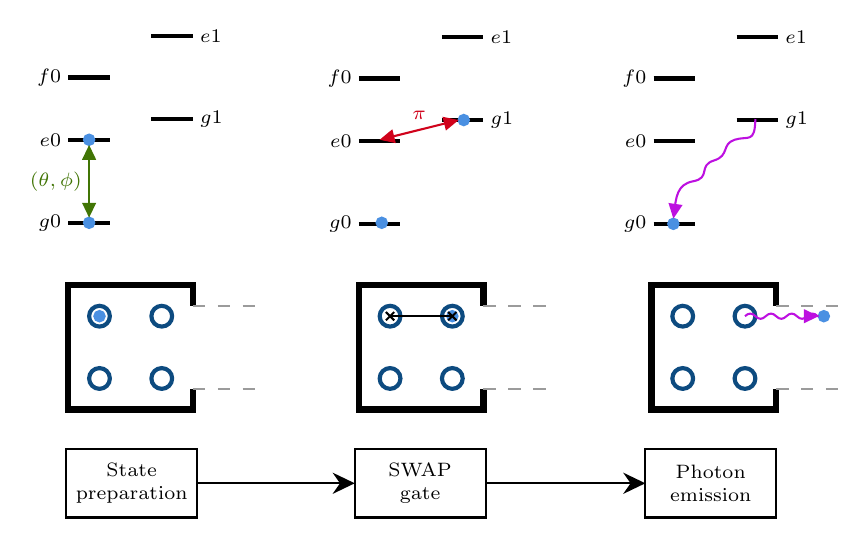
\begin{tikzpicture}[x=0.75pt,y=0.75pt,yscale=-1,xscale=1]
%uncomment if require: \path (0,472); %set diagram left start at 0, and has height of 472

%Straight Lines [id:da8931975658515314] 
\draw [line width=1.5]    (100,100) -- (120,100) ;
%Straight Lines [id:da6109179246921593] 
\draw [line width=1.5]    (140,80) -- (160,80) ;
%Straight Lines [id:da4740245259238267] 
\draw [line width=1.5]    (100,130) -- (120,130) ;
%Straight Lines [id:da8570593937301805] 
\draw [line width=1.5]    (100,170) -- (120,170) ;
%Straight Lines [id:da02915524605611408] 
\draw [line width=1.5]    (140,120) -- (160,120) ;
%Straight Lines [id:da16734412566121315] 
\draw [line width=1.5]    (240,100.5) -- (260,100.5) ;
%Straight Lines [id:da1741824563512493] 
\draw [line width=1.5]    (280,80.5) -- (300,80.5) ;
%Straight Lines [id:da23317779450869036] 
\draw [line width=1.5]    (240,130.5) -- (260,130.5) ;
%Straight Lines [id:da8493304549912968] 
\draw [line width=1.5]    (240,170.5) -- (260,170.5) ;
%Straight Lines [id:da9896717165480059] 
\draw [line width=1.5]    (280,120.5) -- (300,120.5) ;
%Straight Lines [id:da956624069338186] 
\draw [line width=1.5]    (382,100.5) -- (402,100.5) ;
%Straight Lines [id:da7887267818588047] 
\draw [line width=1.5]    (422,80.5) -- (442,80.5) ;
%Straight Lines [id:da03622865125847419] 
\draw [line width=1.5]    (382,130.5) -- (402,130.5) ;
%Straight Lines [id:da13614260982775128] 
\draw [line width=1.5]    (382,170.5) -- (402,170.5) ;
%Straight Lines [id:da1441695211618249] 
\draw [line width=1.5]    (422,120.5) -- (442,120.5) ;
%Shape: Circle [id:dp1759227411497647] 
\draw  [color={rgb, 255:red, 13; green, 75; blue, 128 }  ,draw opacity=1 ][line width=1.5]  (110,215) .. controls (110,212.24) and (112.24,210) .. (115,210) .. controls (117.76,210) and (120,212.24) .. (120,215) .. controls (120,217.76) and (117.76,220) .. (115,220) .. controls (112.24,220) and (110,217.76) .. (110,215) -- cycle ;
%Shape: Circle [id:dp4360171288549991] 
\draw  [color={rgb, 255:red, 13; green, 75; blue, 128 }  ,draw opacity=1 ][line width=1.5]  (110,245) .. controls (110,242.24) and (112.24,240) .. (115,240) .. controls (117.76,240) and (120,242.24) .. (120,245) .. controls (120,247.76) and (117.76,250) .. (115,250) .. controls (112.24,250) and (110,247.76) .. (110,245) -- cycle ;
%Shape: Circle [id:dp5194230164195629] 
\draw  [color={rgb, 255:red, 13; green, 75; blue, 128 }  ,draw opacity=1 ][line width=1.5]  (140,245) .. controls (140,242.24) and (142.24,240) .. (145,240) .. controls (147.76,240) and (150,242.24) .. (150,245) .. controls (150,247.76) and (147.76,250) .. (145,250) .. controls (142.24,250) and (140,247.76) .. (140,245) -- cycle ;
%Shape: Circle [id:dp7655825363179872] 
\draw  [color={rgb, 255:red, 13; green, 75; blue, 128 }  ,draw opacity=1 ][line width=1.5]  (140,215) .. controls (140,212.24) and (142.24,210) .. (145,210) .. controls (147.76,210) and (150,212.24) .. (150,215) .. controls (150,217.76) and (147.76,220) .. (145,220) .. controls (142.24,220) and (140,217.76) .. (140,215) -- cycle ;
%Shape: Square [id:dp010299027105199587] 
\draw  [line width=2.25]  (100,200) -- (160,200) -- (160,260) -- (100,260) -- cycle ;
%Straight Lines [id:da10238522924376559] 
\draw [color={rgb, 255:red, 255; green, 255; blue, 255 }  ,draw opacity=1 ][line width=3]    (160,210) -- (160,250) ;

%Shape: Circle [id:dp042388463572761714] 
\draw  [color={rgb, 255:red, 74; green, 144; blue, 226 }  ,draw opacity=1 ][fill={rgb, 255:red, 74; green, 144; blue, 226 }  ,fill opacity=1 ] (112.5,215) .. controls (112.5,213.62) and (113.62,212.5) .. (115,212.5) .. controls (116.38,212.5) and (117.5,213.62) .. (117.5,215) .. controls (117.5,216.38) and (116.38,217.5) .. (115,217.5) .. controls (113.62,217.5) and (112.5,216.38) .. (112.5,215) -- cycle ;
%Shape: Circle [id:dp10905807386965438] 
\draw  [color={rgb, 255:red, 13; green, 75; blue, 128 }  ,draw opacity=1 ][line width=1.5]  (250,215) .. controls (250,212.24) and (252.24,210) .. (255,210) .. controls (257.76,210) and (260,212.24) .. (260,215) .. controls (260,217.76) and (257.76,220) .. (255,220) .. controls (252.24,220) and (250,217.76) .. (250,215) -- cycle ;
%Shape: Circle [id:dp1368955719904016] 
\draw  [color={rgb, 255:red, 13; green, 75; blue, 128 }  ,draw opacity=1 ][line width=1.5]  (250,245) .. controls (250,242.24) and (252.24,240) .. (255,240) .. controls (257.76,240) and (260,242.24) .. (260,245) .. controls (260,247.76) and (257.76,250) .. (255,250) .. controls (252.24,250) and (250,247.76) .. (250,245) -- cycle ;
%Shape: Circle [id:dp9583422679674527] 
\draw  [color={rgb, 255:red, 13; green, 75; blue, 128 }  ,draw opacity=1 ][line width=1.5]  (280,245) .. controls (280,242.24) and (282.24,240) .. (285,240) .. controls (287.76,240) and (290,242.24) .. (290,245) .. controls (290,247.76) and (287.76,250) .. (285,250) .. controls (282.24,250) and (280,247.76) .. (280,245) -- cycle ;
%Shape: Circle [id:dp6563593124398152] 
\draw  [color={rgb, 255:red, 13; green, 75; blue, 128 }  ,draw opacity=1 ][line width=1.5]  (280,215) .. controls (280,212.24) and (282.24,210) .. (285,210) .. controls (287.76,210) and (290,212.24) .. (290,215) .. controls (290,217.76) and (287.76,220) .. (285,220) .. controls (282.24,220) and (280,217.76) .. (280,215) -- cycle ;
%Shape: Square [id:dp13654534966408327] 
\draw  [line width=2.25]  (240,200) -- (300,200) -- (300,260) -- (240,260) -- cycle ;
%Straight Lines [id:da4280868328748867] 
\draw [color={rgb, 255:red, 255; green, 255; blue, 255 }  ,draw opacity=1 ][line width=3]    (300,210) -- (300,250) ;

%Shape: Circle [id:dp3843313988885617] 
\draw  [color={rgb, 255:red, 74; green, 144; blue, 226 }  ,draw opacity=1 ][fill={rgb, 255:red, 74; green, 144; blue, 226 }  ,fill opacity=1 ] (282.5,215) .. controls (282.5,213.62) and (283.62,212.5) .. (285,212.5) .. controls (286.38,212.5) and (287.5,213.62) .. (287.5,215) .. controls (287.5,216.38) and (286.38,217.5) .. (285,217.5) .. controls (283.62,217.5) and (282.5,216.38) .. (282.5,215) -- cycle ;
%Shape: Circle [id:dp9771460101503161] 
\draw  [color={rgb, 255:red, 13; green, 75; blue, 128 }  ,draw opacity=1 ][line width=1.5]  (391,215) .. controls (391,212.24) and (393.24,210) .. (396,210) .. controls (398.76,210) and (401,212.24) .. (401,215) .. controls (401,217.76) and (398.76,220) .. (396,220) .. controls (393.24,220) and (391,217.76) .. (391,215) -- cycle ;
%Shape: Circle [id:dp504285258273425] 
\draw  [color={rgb, 255:red, 13; green, 75; blue, 128 }  ,draw opacity=1 ][line width=1.5]  (391,245) .. controls (391,242.24) and (393.24,240) .. (396,240) .. controls (398.76,240) and (401,242.24) .. (401,245) .. controls (401,247.76) and (398.76,250) .. (396,250) .. controls (393.24,250) and (391,247.76) .. (391,245) -- cycle ;
%Shape: Circle [id:dp35978571349256916] 
\draw  [color={rgb, 255:red, 13; green, 75; blue, 128 }  ,draw opacity=1 ][line width=1.5]  (421,245) .. controls (421,242.24) and (423.24,240) .. (426,240) .. controls (428.76,240) and (431,242.24) .. (431,245) .. controls (431,247.76) and (428.76,250) .. (426,250) .. controls (423.24,250) and (421,247.76) .. (421,245) -- cycle ;
%Shape: Circle [id:dp48609503948401167] 
\draw  [color={rgb, 255:red, 13; green, 75; blue, 128 }  ,draw opacity=1 ][line width=1.5]  (421,215) .. controls (421,212.24) and (423.24,210) .. (426,210) .. controls (428.76,210) and (431,212.24) .. (431,215) .. controls (431,217.76) and (428.76,220) .. (426,220) .. controls (423.24,220) and (421,217.76) .. (421,215) -- cycle ;
%Shape: Square [id:dp7113243311612103] 
\draw  [line width=2.25]  (381,200) -- (441,200) -- (441,260) -- (381,260) -- cycle ;
%Straight Lines [id:da41970234088616587] 
\draw [color={rgb, 255:red, 255; green, 255; blue, 255 }  ,draw opacity=1 ][line width=3]    (441,210) -- (441,250) ;

%Shape: Circle [id:dp888719115154261] 
\draw  [color={rgb, 255:red, 74; green, 144; blue, 226 }  ,draw opacity=1 ][fill={rgb, 255:red, 74; green, 144; blue, 226 }  ,fill opacity=1 ] (461.5,215) .. controls (461.5,213.62) and (462.62,212.5) .. (464,212.5) .. controls (465.38,212.5) and (466.5,213.62) .. (466.5,215) .. controls (466.5,216.38) and (465.38,217.5) .. (464,217.5) .. controls (462.62,217.5) and (461.5,216.38) .. (461.5,215) -- cycle ;
%Shape: Circle [id:dp5496267038959322] 
\draw  [color={rgb, 255:red, 74; green, 144; blue, 226 }  ,draw opacity=1 ][fill={rgb, 255:red, 74; green, 144; blue, 226 }  ,fill opacity=1 ] (107.5,170) .. controls (107.5,168.62) and (108.62,167.5) .. (110,167.5) .. controls (111.38,167.5) and (112.5,168.62) .. (112.5,170) .. controls (112.5,171.38) and (111.38,172.5) .. (110,172.5) .. controls (108.62,172.5) and (107.5,171.38) .. (107.5,170) -- cycle ;
%Shape: Circle [id:dp16614467553508028] 
\draw  [color={rgb, 255:red, 74; green, 144; blue, 226 }  ,draw opacity=1 ][fill={rgb, 255:red, 74; green, 144; blue, 226 }  ,fill opacity=1 ] (107.5,130) .. controls (107.5,128.62) and (108.62,127.5) .. (110,127.5) .. controls (111.38,127.5) and (112.5,128.62) .. (112.5,130) .. controls (112.5,131.38) and (111.38,132.5) .. (110,132.5) .. controls (108.62,132.5) and (107.5,131.38) .. (107.5,130) -- cycle ;
%Straight Lines [id:da761425443907652] 
\draw [color={rgb, 255:red, 65; green, 117; blue, 5 }  ,draw opacity=1 ]   (110,135.5) -- (110,164.5) ;
\draw [shift={(110,167.5)}, rotate = 270] [fill={rgb, 255:red, 65; green, 117; blue, 5 }  ,fill opacity=1 ][line width=0.08]  [draw opacity=0] (7.14,-3.43) -- (0,0) -- (7.14,3.43) -- cycle    ;
\draw [shift={(110,132.5)}, rotate = 90] [fill={rgb, 255:red, 65; green, 117; blue, 5 }  ,fill opacity=1 ][line width=0.08]  [draw opacity=0] (7.14,-3.43) -- (0,0) -- (7.14,3.43) -- cycle    ;
%Shape: Circle [id:dp38814788928849464] 
\draw  [color={rgb, 255:red, 74; green, 144; blue, 226 }  ,draw opacity=1 ][fill={rgb, 255:red, 74; green, 144; blue, 226 }  ,fill opacity=1 ] (248.5,170) .. controls (248.5,168.62) and (249.62,167.5) .. (251,167.5) .. controls (252.38,167.5) and (253.5,168.62) .. (253.5,170) .. controls (253.5,171.38) and (252.38,172.5) .. (251,172.5) .. controls (249.62,172.5) and (248.5,171.38) .. (248.5,170) -- cycle ;
%Shape: Circle [id:dp40578346278756805] 
\draw  [color={rgb, 255:red, 74; green, 144; blue, 226 }  ,draw opacity=1 ][fill={rgb, 255:red, 74; green, 144; blue, 226 }  ,fill opacity=1 ] (288,120.5) .. controls (288,119.12) and (289.12,118) .. (290.5,118) .. controls (291.88,118) and (293,119.12) .. (293,120.5) .. controls (293,121.88) and (291.88,123) .. (290.5,123) .. controls (289.12,123) and (288,121.88) .. (288,120.5) -- cycle ;
%Straight Lines [id:da9874028184585202] 
\draw [color={rgb, 255:red, 208; green, 2; blue, 27 }  ,draw opacity=1 ]   (252.91,129.27) -- (285.09,121.23) ;
\draw [shift={(288,120.5)}, rotate = 165.96] [fill={rgb, 255:red, 208; green, 2; blue, 27 }  ,fill opacity=1 ][line width=0.08]  [draw opacity=0] (7.14,-3.43) -- (0,0) -- (7.14,3.43) -- cycle    ;
\draw [shift={(250,130)}, rotate = 345.96] [fill={rgb, 255:red, 208; green, 2; blue, 27 }  ,fill opacity=1 ][line width=0.08]  [draw opacity=0] (7.14,-3.43) -- (0,0) -- (7.14,3.43) -- cycle    ;
%Straight Lines [id:da8925388175427755] 
\draw    (283,213) -- (287,217) ;
%Straight Lines [id:da29737665357676757] 
\draw    (287,213) -- (283,217) ;
%Straight Lines [id:da44962743138305683] 
\draw    (257,213) -- (253,217) ;
%Straight Lines [id:da24591300628760293] 
\draw    (253,213) -- (257,217) ;
%Straight Lines [id:da7218180056220298] 
\draw    (255,215) -- (285,215) ;
%Shape: Circle [id:dp8443381413544921] 
\draw  [color={rgb, 255:red, 74; green, 144; blue, 226 }  ,draw opacity=1 ][fill={rgb, 255:red, 74; green, 144; blue, 226 }  ,fill opacity=1 ] (389,170.5) .. controls (389,169.12) and (390.12,168) .. (391.5,168) .. controls (392.88,168) and (394,169.12) .. (394,170.5) .. controls (394,171.88) and (392.88,173) .. (391.5,173) .. controls (390.12,173) and (389,171.88) .. (389,170.5) -- cycle ;
%Curve Lines [id:da9123421404371583] 
\draw [color={rgb, 255:red, 189; green, 16; blue, 224 }  ,draw opacity=1 ]   (431,120) .. controls (430.75,132.13) and (427.5,127.88) .. (421,130) .. controls (414.5,132.13) and (418.75,137.63) .. (411,140) .. controls (403.25,142.38) and (409.75,148.38) .. (401,150) .. controls (393.26,151.44) and (392.76,157.67) .. (391.88,165.07) ;
\draw [shift={(391.5,168)}, rotate = 278.25] [fill={rgb, 255:red, 189; green, 16; blue, 224 }  ,fill opacity=1 ][line width=0.08]  [draw opacity=0] (7.14,-3.43) -- (0,0) -- (7.14,3.43) -- cycle    ;
%Straight Lines [id:da3528583271662068] 
\draw [color={rgb, 255:red, 155; green, 155; blue, 155 }  ,draw opacity=1 ] [dash pattern={on 4.5pt off 4.5pt}]  (160,210) -- (190,210) ;
%Straight Lines [id:da7594522783532085] 
\draw [color={rgb, 255:red, 189; green, 16; blue, 224 }  ,draw opacity=1 ]   (426,215) .. controls (427.67,213.33) and (429.33,213.33) .. (431,215) .. controls (432.67,216.67) and (434.33,216.67) .. (436,215) .. controls (437.67,213.33) and (439.33,213.33) .. (441,215) .. controls (442.67,216.67) and (444.33,216.67) .. (446,215) .. controls (447.67,213.33) and (449.33,213.33) .. (451,215) .. controls (452.67,216.67) and (454.33,216.67) .. (456,215) .. controls (457.67,213.33) and (459.33,213.33) .. (461,215) -- (461.5,215) -- (461.5,215) ;
%Straight Lines [id:da7501083613796489] 
\draw [color={rgb, 255:red, 155; green, 155; blue, 155 }  ,draw opacity=1 ] [dash pattern={on 4.5pt off 4.5pt}]  (160,250) -- (190,250) ;
%Straight Lines [id:da7402563943632688] 
\draw [color={rgb, 255:red, 155; green, 155; blue, 155 }  ,draw opacity=1 ] [dash pattern={on 4.5pt off 4.5pt}]  (441,210) -- (471,210) ;
%Straight Lines [id:da36408062706405653] 
\draw [color={rgb, 255:red, 155; green, 155; blue, 155 }  ,draw opacity=1 ] [dash pattern={on 4.5pt off 4.5pt}]  (441,250) -- (471,250) ;
%Straight Lines [id:da0547231990275685] 
\draw [color={rgb, 255:red, 155; green, 155; blue, 155 }  ,draw opacity=1 ] [dash pattern={on 4.5pt off 4.5pt}]  (300,210) -- (330,210) ;
%Straight Lines [id:da7486275799999674] 
\draw [color={rgb, 255:red, 155; green, 155; blue, 155 }  ,draw opacity=1 ] [dash pattern={on 4.5pt off 4.5pt}]  (300,250) -- (330,250) ;
%Straight Lines [id:da691181939054564] 
\draw [color={rgb, 255:red, 189; green, 16; blue, 224 }  ,draw opacity=1 ]   (455.75,215) -- (458.5,215) ;
\draw [shift={(461.5,215)}, rotate = 180] [fill={rgb, 255:red, 189; green, 16; blue, 224 }  ,fill opacity=1 ][line width=0.08]  [draw opacity=0] (7.14,-3.43) -- (0,0) -- (7.14,3.43) -- cycle    ;

% Text Node
\draw (98,100) node [anchor=east] [inner sep=0.75pt]  [font=\scriptsize]  {$f0$};
% Text Node
\draw (98,130) node [anchor=east] [inner sep=0.75pt]  [font=\scriptsize]  {$e0$};
% Text Node
\draw (98,170) node [anchor=east] [inner sep=0.75pt]  [font=\scriptsize]  {$g0$};
% Text Node
\draw (162,80) node [anchor=west] [inner sep=0.75pt]  [font=\scriptsize]  {$e1$};
% Text Node
\draw (162,120) node [anchor=west] [inner sep=0.75pt]  [font=\scriptsize]  {$g1$};
% Text Node
\draw (238,100.5) node [anchor=east] [inner sep=0.75pt]  [font=\scriptsize]  {$f0$};
% Text Node
\draw (238,130.5) node [anchor=east] [inner sep=0.75pt]  [font=\scriptsize]  {$e0$};
% Text Node
\draw (238,170.5) node [anchor=east] [inner sep=0.75pt]  [font=\scriptsize]  {$g0$};
% Text Node
\draw (302,80.5) node [anchor=west] [inner sep=0.75pt]  [font=\scriptsize]  {$e1$};
% Text Node
\draw (302,120.5) node [anchor=west] [inner sep=0.75pt]  [font=\scriptsize]  {$g1$};
% Text Node
\draw (380,100.5) node [anchor=east] [inner sep=0.75pt]  [font=\scriptsize]  {$f0$};
% Text Node
\draw (380,130.5) node [anchor=east] [inner sep=0.75pt]  [font=\scriptsize]  {$e0$};
% Text Node
\draw (380,170.5) node [anchor=east] [inner sep=0.75pt]  [font=\scriptsize]  {$g0$};
% Text Node
\draw (444,80.5) node [anchor=west] [inner sep=0.75pt]  [font=\scriptsize]  {$e1$};
% Text Node
\draw (444,120.5) node [anchor=west] [inner sep=0.75pt]  [font=\scriptsize]  {$g1$};
% Text Node
\draw (108,150) node [anchor=east] [inner sep=0.75pt]  [font=\scriptsize,color={rgb, 255:red, 65; green, 117; blue, 5 }  ,opacity=1 ]  {$( \theta ,\phi )$};
% Text Node
\draw (269,121.85) node [anchor=south] [inner sep=0.75pt]  [font=\scriptsize,color={rgb, 255:red, 208; green, 2; blue, 27 }  ,opacity=1 ]  {$\pi $};
% Text Node
\draw    (99,279) -- (162,279) -- (162,312) -- (99,312) -- cycle  ;
\draw (130.5,295.5) node  [font=\scriptsize] [align=left] {\begin{minipage}[lt]{40.8pt}\setlength\topsep{0pt}
\begin{center}
State preparation
\end{center}

\end{minipage}};
% Text Node
\draw    (238,279) -- (301,279) -- (301,312) -- (238,312) -- cycle  ;
\draw (269.5,295.5) node  [font=\scriptsize] [align=left] {\begin{minipage}[lt]{40.8pt}\setlength\topsep{0pt}
\begin{center}
SWAP\\gate
\end{center}

\end{minipage}};
% Text Node
\draw    (378,279) -- (441,279) -- (441,312) -- (378,312) -- cycle  ;
\draw (409.5,295.5) node  [font=\scriptsize] [align=left] {\begin{minipage}[lt]{40.8pt}\setlength\topsep{0pt}
\begin{center}
Photon\\emission
\end{center}

\end{minipage}};
% Connection
\draw    (162,295.5) -- (235,295.5) ;
\draw [shift={(238,295.5)}, rotate = 180] [fill={rgb, 255:red, 0; green, 0; blue, 0 }  ][line width=0.08]  [draw opacity=0] (10.72,-5.15) -- (0,0) -- (10.72,5.15) -- (7.12,0) -- cycle    ;
% Connection
\draw    (301,295.5) -- (375,295.5) ;
\draw [shift={(378,295.5)}, rotate = 180] [fill={rgb, 255:red, 0; green, 0; blue, 0 }  ][line width=0.08]  [draw opacity=0] (10.72,-5.15) -- (0,0) -- (10.72,5.15) -- (7.12,0) -- cycle    ;

\end{tikzpicture}
    \vspace{-1cm}
    \caption{Protocol for executing an S-E SWAP gate}
    \label{fig:S-E_SWAP}
\end{figure}

The depicted sequence shown in \cref{fig:S-E_SWAP} illustrates the operations required to execute the SWAP gate between a storage and an emitter.
First, an arbitrary state is prepared on the storage qubit through single-qubit operations.
Following this, a $\pi$ rotation is induced within the $e0$-$g1$ manifold of the two-qubit system.
Lastly, upon decay of the emitter qubit, a photon is emitted in the emission line, preserving the state initially encoded by the storage qubit.

In the protocol described before, the interaction between the qubits is switched on to execute the $\pi$ rotation between the $e0$ and the $g1$ energy levels of the two-qubit gate.
We thus need to calibrate this operation using \cref{eq:chevron_kappa}, obtained from the previous discussion on modelling the interaction in the presence of an external decay channel.
Figure~\ref{fig:SWAP_chevrons} shows the data taken to calibrate the $\pi$ rotation in the $e0$-$g1$ manifold.
The data is then fit to the model in order to get the operational point, depicted as a dot in the figure.
The waiting time in order to achieve the desired gate is given by
\begin{equation}
\label{eq:tilde_t_kappa}
    \widetilde{t} = 2 \cdot \frac{\pi - \arctan(2 \Omega / \kappa )}{\Omega} ,
\end{equation}
where $\Omega$ is given by \cref{eq:eff_Raby_kappa}.

\begin{figure}
    \centering
    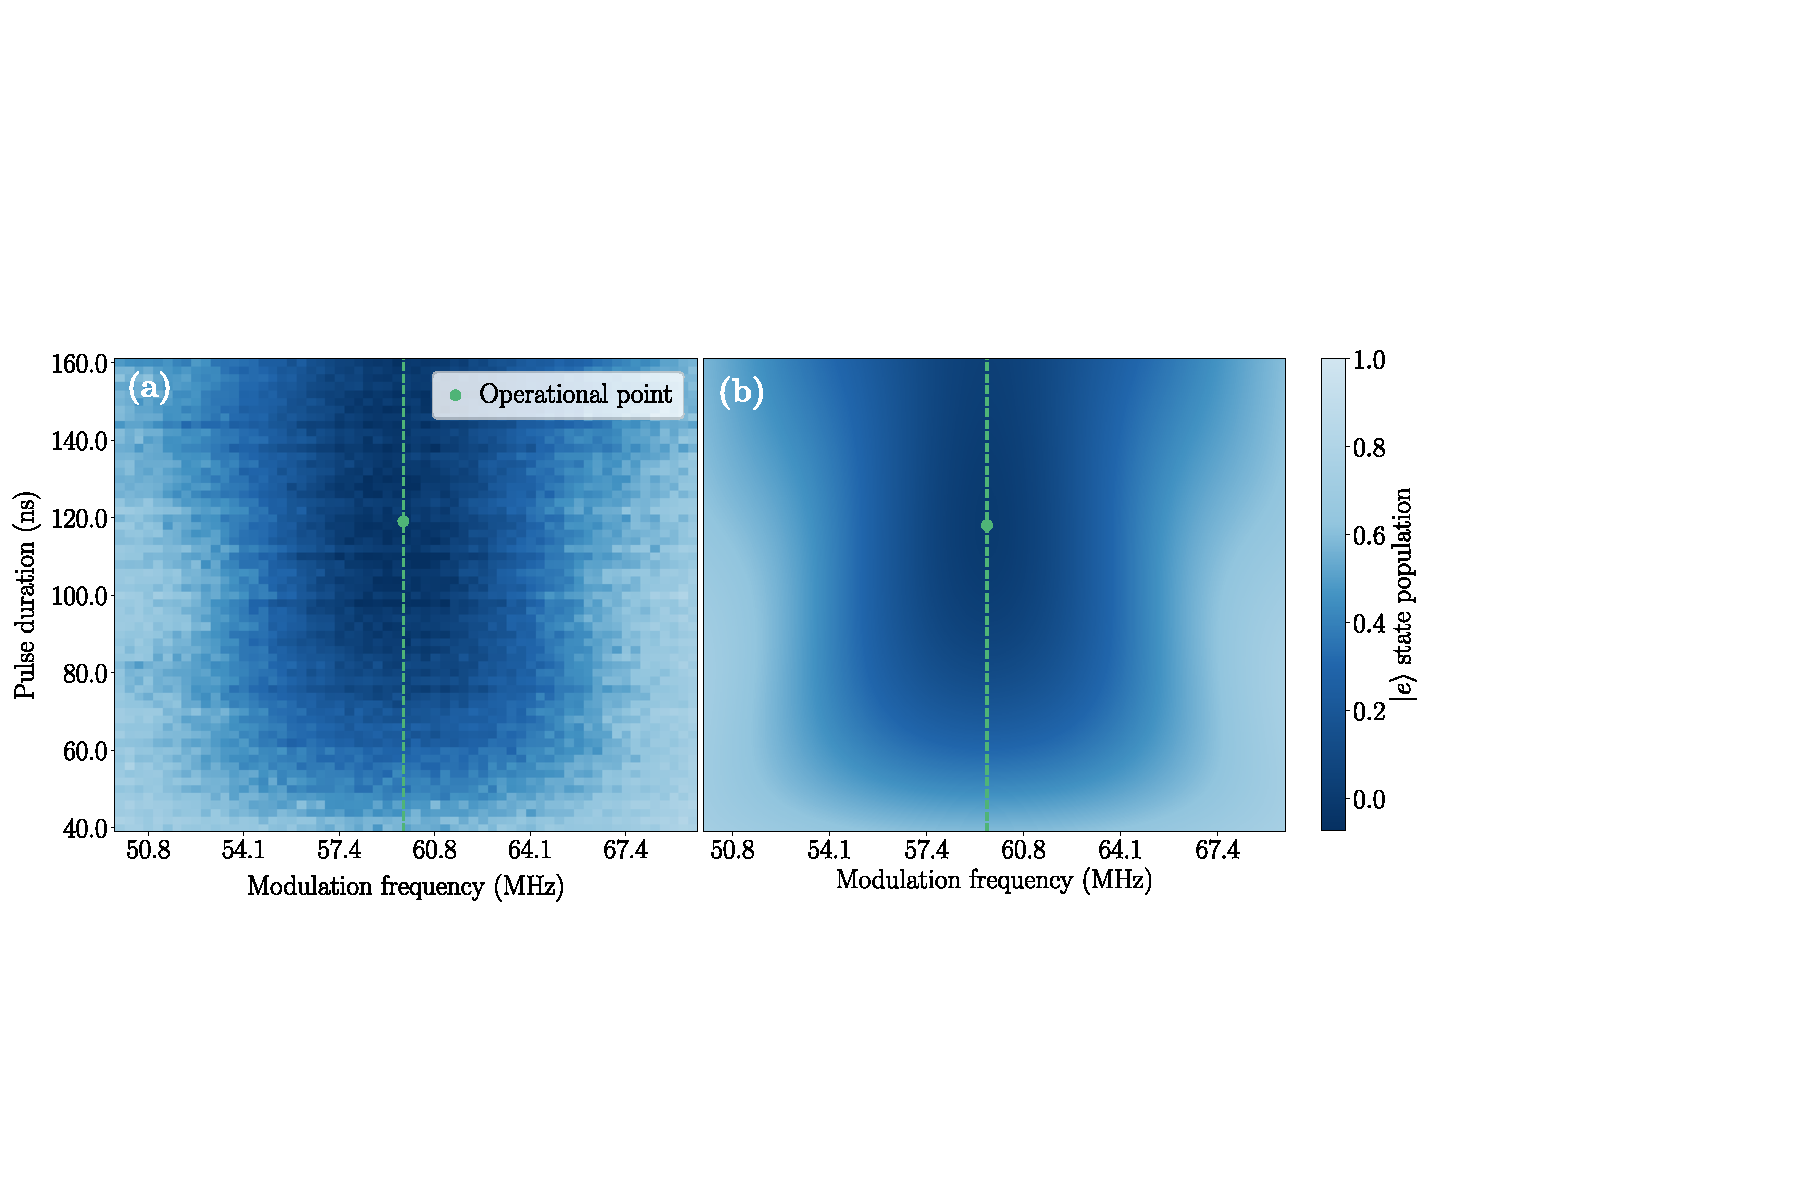
\includegraphics[width = \textwidth]{Images/Chap3/a.pdf}
    \caption{\textbf{(a)} data of the $e0g1$ transition within a storage-emitter pair with \textbf{(b)} relative fit}
    \label{fig:SWAP_chevrons}
\end{figure}

Before initiating each new protocol, it is essential to reset the population of the storage qubits.
This can be achieved through either passive waiting or by executing the resetting protocol.
Since the emitter qubit can be assured to be in the ground state, we just transfer the excitation from the storage to the respective emitter qubit, which subsequently releases them into the emission line.
In theory, achieving this could involve simply executing a SWAP gate.
However, in practice, we observe improved performance by prolonging the $e0$-$g1$ transition.
This approach achieves the desired outcome of resetting the storage qubit state to the ground state $\ket{g}$.

\subsection{CNOT}

The other operation that we can run between storage and emitter qubits is a controlled emission, or CNOT.
The unitary matrix representing this operation is
\begin{equation}
    U_{\text{CNOT}} = 
    \begin{pmatrix}
    1 & 0 & 0 & 0 \\
    0 & 1 & 0 & 0 \\
    0 & 0 & 0 & 1 \\
    0 & 0 & 1 & 0 \\
\end{pmatrix}.
\end{equation}

A photon is emitted from the emitter qubit only if the storage qubit is in the excited state $\ket{e}$, otherwise no photon is emitted.
Thus, it performs the operation
\begin{equation}
    \ket{\psi}_{\text{S}} \ket{0}_{\text{E}} = 
    (\alpha \ket{g0} + \beta \ket{e0})_{\text{SE}} \xrightarrow{U_{\text{CNOT}}}
    (\alpha \ket{g0} + \beta \ket{e1})_{\text{SE}} .
\end{equation}

Note that, since the final state cannot be expressed as a tensor product of two individual pure states, the resulting state is entangled.

\begin{figure}
    \centering
    

\tikzset{every picture/.style={line width=0.75pt}} %set default line width to 0.75pt        

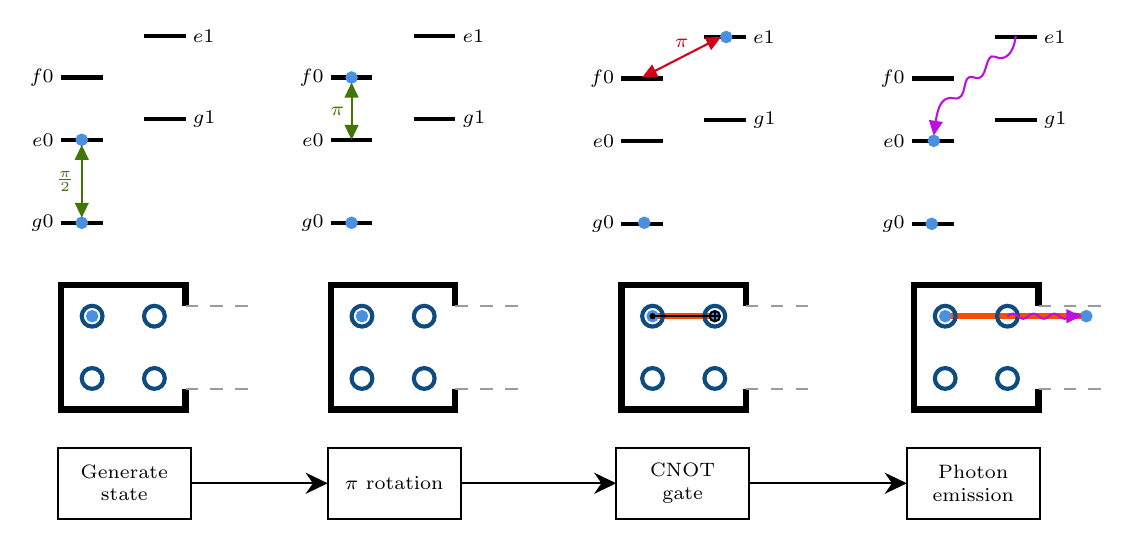
\begin{tikzpicture}[x=0.75pt,y=0.75pt,yscale=-1,xscale=1]
%uncomment if require: \path (0,369); %set diagram left start at 0, and has height of 369

%Shape: Square [id:dp16311871674784617] 
\draw  [line width=2.25]  (451,200) -- (511,200) -- (511,260) -- (451,260) -- cycle ;
%Straight Lines [id:da7729927634660387] 
\draw [color={rgb, 255:red, 255; green, 255; blue, 255 }  ,draw opacity=1 ][line width=3]    (511,210) -- (511,250) ;

%Straight Lines [id:da7800146811047701] 
\draw [color={rgb, 255:red, 246; green, 76; blue, 4 }  ,draw opacity=1 ][line width=2.25]    (466,215) -- (534,215) ;
%Straight Lines [id:da6261448047007223] 
\draw [color={rgb, 255:red, 246; green, 76; blue, 4 }  ,draw opacity=1 ][line width=2.25]    (325,215) -- (355,215) ;
%Shape: Circle [id:dp08255337848175437] 
\draw  [color={rgb, 255:red, 74; green, 144; blue, 226 }  ,draw opacity=1 ][fill={rgb, 255:red, 74; green, 144; blue, 226 }  ,fill opacity=1 ] (322.5,215) .. controls (322.5,213.62) and (323.62,212.5) .. (325,212.5) .. controls (326.38,212.5) and (327.5,213.62) .. (327.5,215) .. controls (327.5,216.38) and (326.38,217.5) .. (325,217.5) .. controls (323.62,217.5) and (322.5,216.38) .. (322.5,215) -- cycle ;
%Straight Lines [id:da9104352429816489] 
\draw [line width=1.5]    (170,100) -- (190,100) ;
%Straight Lines [id:da4044326119304753] 
\draw [line width=1.5]    (210,80) -- (230,80) ;
%Straight Lines [id:da8246098672675921] 
\draw [line width=1.5]    (170,130) -- (190,130) ;
%Straight Lines [id:da28026964700411405] 
\draw [line width=1.5]    (170,170) -- (190,170) ;
%Straight Lines [id:da6372847917499911] 
\draw [line width=1.5]    (210,120) -- (230,120) ;
%Straight Lines [id:da7158175267683015] 
\draw [line width=1.5]    (310,100.5) -- (330,100.5) ;
%Straight Lines [id:da029189986581482863] 
\draw [line width=1.5]    (350,80.5) -- (370,80.5) ;
%Straight Lines [id:da5055762916284449] 
\draw [line width=1.5]    (310,130.5) -- (330,130.5) ;
%Straight Lines [id:da12540512017651273] 
\draw [line width=1.5]    (310,170.5) -- (330,170.5) ;
%Straight Lines [id:da6841661375720638] 
\draw [line width=1.5]    (350,120.5) -- (370,120.5) ;
%Straight Lines [id:da07667408340673776] 
\draw [line width=1.5]    (450,100.5) -- (470,100.5) ;
%Straight Lines [id:da5408805406645967] 
\draw [line width=1.5]    (490,80.5) -- (510,80.5) ;
%Straight Lines [id:da29633743286868486] 
\draw [line width=1.5]    (450,130.5) -- (470,130.5) ;
%Straight Lines [id:da4224256257765836] 
\draw [line width=1.5]    (450,170.5) -- (470,170.5) ;
%Straight Lines [id:da5748015229993475] 
\draw [line width=1.5]    (490,120.5) -- (510,120.5) ;
%Shape: Circle [id:dp17205385892315683] 
\draw  [color={rgb, 255:red, 13; green, 75; blue, 128 }  ,draw opacity=1 ][line width=1.5]  (180,215) .. controls (180,212.24) and (182.24,210) .. (185,210) .. controls (187.76,210) and (190,212.24) .. (190,215) .. controls (190,217.76) and (187.76,220) .. (185,220) .. controls (182.24,220) and (180,217.76) .. (180,215) -- cycle ;
%Shape: Circle [id:dp31352659886469914] 
\draw  [color={rgb, 255:red, 13; green, 75; blue, 128 }  ,draw opacity=1 ][line width=1.5]  (180,245) .. controls (180,242.24) and (182.24,240) .. (185,240) .. controls (187.76,240) and (190,242.24) .. (190,245) .. controls (190,247.76) and (187.76,250) .. (185,250) .. controls (182.24,250) and (180,247.76) .. (180,245) -- cycle ;
%Shape: Circle [id:dp5992292171552074] 
\draw  [color={rgb, 255:red, 13; green, 75; blue, 128 }  ,draw opacity=1 ][line width=1.5]  (210,245) .. controls (210,242.24) and (212.24,240) .. (215,240) .. controls (217.76,240) and (220,242.24) .. (220,245) .. controls (220,247.76) and (217.76,250) .. (215,250) .. controls (212.24,250) and (210,247.76) .. (210,245) -- cycle ;
%Shape: Circle [id:dp5175687516944736] 
\draw  [color={rgb, 255:red, 13; green, 75; blue, 128 }  ,draw opacity=1 ][line width=1.5]  (210,215) .. controls (210,212.24) and (212.24,210) .. (215,210) .. controls (217.76,210) and (220,212.24) .. (220,215) .. controls (220,217.76) and (217.76,220) .. (215,220) .. controls (212.24,220) and (210,217.76) .. (210,215) -- cycle ;
%Shape: Square [id:dp7278738414250778] 
\draw  [line width=2.25]  (170,200) -- (230,200) -- (230,260) -- (170,260) -- cycle ;
%Straight Lines [id:da27484081993709997] 
\draw [color={rgb, 255:red, 255; green, 255; blue, 255 }  ,draw opacity=1 ][line width=3]    (230,210) -- (230,250) ;

%Shape: Circle [id:dp7417447571645056] 
\draw  [color={rgb, 255:red, 74; green, 144; blue, 226 }  ,draw opacity=1 ][fill={rgb, 255:red, 74; green, 144; blue, 226 }  ,fill opacity=1 ] (182.5,215) .. controls (182.5,213.62) and (183.62,212.5) .. (185,212.5) .. controls (186.38,212.5) and (187.5,213.62) .. (187.5,215) .. controls (187.5,216.38) and (186.38,217.5) .. (185,217.5) .. controls (183.62,217.5) and (182.5,216.38) .. (182.5,215) -- cycle ;
%Shape: Circle [id:dp5521220556000415] 
\draw  [color={rgb, 255:red, 13; green, 75; blue, 128 }  ,draw opacity=1 ][line width=1.5]  (320,215) .. controls (320,212.24) and (322.24,210) .. (325,210) .. controls (327.76,210) and (330,212.24) .. (330,215) .. controls (330,217.76) and (327.76,220) .. (325,220) .. controls (322.24,220) and (320,217.76) .. (320,215) -- cycle ;
%Shape: Circle [id:dp5119802656626787] 
\draw  [color={rgb, 255:red, 13; green, 75; blue, 128 }  ,draw opacity=1 ][line width=1.5]  (320,245) .. controls (320,242.24) and (322.24,240) .. (325,240) .. controls (327.76,240) and (330,242.24) .. (330,245) .. controls (330,247.76) and (327.76,250) .. (325,250) .. controls (322.24,250) and (320,247.76) .. (320,245) -- cycle ;
%Shape: Circle [id:dp45831332554801185] 
\draw  [color={rgb, 255:red, 13; green, 75; blue, 128 }  ,draw opacity=1 ][line width=1.5]  (350,245) .. controls (350,242.24) and (352.24,240) .. (355,240) .. controls (357.76,240) and (360,242.24) .. (360,245) .. controls (360,247.76) and (357.76,250) .. (355,250) .. controls (352.24,250) and (350,247.76) .. (350,245) -- cycle ;
%Shape: Circle [id:dp5667242703643459] 
\draw  [color={rgb, 255:red, 13; green, 75; blue, 128 }  ,draw opacity=1 ][line width=1.5]  (350,215) .. controls (350,212.24) and (352.24,210) .. (355,210) .. controls (357.76,210) and (360,212.24) .. (360,215) .. controls (360,217.76) and (357.76,220) .. (355,220) .. controls (352.24,220) and (350,217.76) .. (350,215) -- cycle ;
%Shape: Square [id:dp8519449086567641] 
\draw  [line width=2.25]  (310,200) -- (370,200) -- (370,260) -- (310,260) -- cycle ;
%Straight Lines [id:da6856000655126234] 
\draw [color={rgb, 255:red, 255; green, 255; blue, 255 }  ,draw opacity=1 ][line width=3]    (370,210) -- (370,250) ;

%Shape: Circle [id:dp20438827688260486] 
\draw  [color={rgb, 255:red, 0; green, 0; blue, 0 }  ,draw opacity=1 ][fill={rgb, 255:red, 74; green, 144; blue, 226 }  ,fill opacity=1 ] (352.5,215) .. controls (352.5,213.62) and (353.62,212.5) .. (355,212.5) .. controls (356.38,212.5) and (357.5,213.62) .. (357.5,215) .. controls (357.5,216.38) and (356.38,217.5) .. (355,217.5) .. controls (353.62,217.5) and (352.5,216.38) .. (352.5,215) -- cycle ;
%Shape: Circle [id:dp5596871069752617] 
\draw  [color={rgb, 255:red, 13; green, 75; blue, 128 }  ,draw opacity=1 ][line width=1.5]  (461,215) .. controls (461,212.24) and (463.24,210) .. (466,210) .. controls (468.76,210) and (471,212.24) .. (471,215) .. controls (471,217.76) and (468.76,220) .. (466,220) .. controls (463.24,220) and (461,217.76) .. (461,215) -- cycle ;
%Shape: Circle [id:dp23654847702851645] 
\draw  [color={rgb, 255:red, 13; green, 75; blue, 128 }  ,draw opacity=1 ][line width=1.5]  (461,245) .. controls (461,242.24) and (463.24,240) .. (466,240) .. controls (468.76,240) and (471,242.24) .. (471,245) .. controls (471,247.76) and (468.76,250) .. (466,250) .. controls (463.24,250) and (461,247.76) .. (461,245) -- cycle ;
%Shape: Circle [id:dp9337844037205707] 
\draw  [color={rgb, 255:red, 13; green, 75; blue, 128 }  ,draw opacity=1 ][line width=1.5]  (491,245) .. controls (491,242.24) and (493.24,240) .. (496,240) .. controls (498.76,240) and (501,242.24) .. (501,245) .. controls (501,247.76) and (498.76,250) .. (496,250) .. controls (493.24,250) and (491,247.76) .. (491,245) -- cycle ;
%Shape: Circle [id:dp9108295407689929] 
\draw  [color={rgb, 255:red, 13; green, 75; blue, 128 }  ,draw opacity=1 ][line width=1.5]  (491,215) .. controls (491,212.24) and (493.24,210) .. (496,210) .. controls (498.76,210) and (501,212.24) .. (501,215) .. controls (501,217.76) and (498.76,220) .. (496,220) .. controls (493.24,220) and (491,217.76) .. (491,215) -- cycle ;
%Shape: Circle [id:dp7135835004027433] 
\draw  [color={rgb, 255:red, 74; green, 144; blue, 226 }  ,draw opacity=1 ][fill={rgb, 255:red, 74; green, 144; blue, 226 }  ,fill opacity=1 ] (531.5,215) .. controls (531.5,213.62) and (532.62,212.5) .. (534,212.5) .. controls (535.38,212.5) and (536.5,213.62) .. (536.5,215) .. controls (536.5,216.38) and (535.38,217.5) .. (534,217.5) .. controls (532.62,217.5) and (531.5,216.38) .. (531.5,215) -- cycle ;
%Shape: Circle [id:dp9013057046264672] 
\draw  [color={rgb, 255:red, 74; green, 144; blue, 226 }  ,draw opacity=1 ][fill={rgb, 255:red, 74; green, 144; blue, 226 }  ,fill opacity=1 ] (177.5,170) .. controls (177.5,168.62) and (178.62,167.5) .. (180,167.5) .. controls (181.38,167.5) and (182.5,168.62) .. (182.5,170) .. controls (182.5,171.38) and (181.38,172.5) .. (180,172.5) .. controls (178.62,172.5) and (177.5,171.38) .. (177.5,170) -- cycle ;
%Shape: Circle [id:dp44633087412727634] 
\draw  [color={rgb, 255:red, 74; green, 144; blue, 226 }  ,draw opacity=1 ][fill={rgb, 255:red, 74; green, 144; blue, 226 }  ,fill opacity=1 ] (177.5,100) .. controls (177.5,98.62) and (178.62,97.5) .. (180,97.5) .. controls (181.38,97.5) and (182.5,98.62) .. (182.5,100) .. controls (182.5,101.38) and (181.38,102.5) .. (180,102.5) .. controls (178.62,102.5) and (177.5,101.38) .. (177.5,100) -- cycle ;
%Straight Lines [id:da7936001347648454] 
\draw [color={rgb, 255:red, 65; green, 117; blue, 5 }  ,draw opacity=1 ]   (180,105.5) -- (180,127) ;
\draw [shift={(180,130)}, rotate = 270] [fill={rgb, 255:red, 65; green, 117; blue, 5 }  ,fill opacity=1 ][line width=0.08]  [draw opacity=0] (7.14,-3.43) -- (0,0) -- (7.14,3.43) -- cycle    ;
\draw [shift={(180,102.5)}, rotate = 90] [fill={rgb, 255:red, 65; green, 117; blue, 5 }  ,fill opacity=1 ][line width=0.08]  [draw opacity=0] (7.14,-3.43) -- (0,0) -- (7.14,3.43) -- cycle    ;
%Shape: Circle [id:dp7488200712756418] 
\draw  [color={rgb, 255:red, 74; green, 144; blue, 226 }  ,draw opacity=1 ][fill={rgb, 255:red, 74; green, 144; blue, 226 }  ,fill opacity=1 ] (318.5,170) .. controls (318.5,168.62) and (319.62,167.5) .. (321,167.5) .. controls (322.38,167.5) and (323.5,168.62) .. (323.5,170) .. controls (323.5,171.38) and (322.38,172.5) .. (321,172.5) .. controls (319.62,172.5) and (318.5,171.38) .. (318.5,170) -- cycle ;
%Shape: Circle [id:dp5107256171224921] 
\draw  [color={rgb, 255:red, 74; green, 144; blue, 226 }  ,draw opacity=1 ][fill={rgb, 255:red, 74; green, 144; blue, 226 }  ,fill opacity=1 ] (358,80.5) .. controls (358,79.12) and (359.12,78) .. (360.5,78) .. controls (361.88,78) and (363,79.12) .. (363,80.5) .. controls (363,81.88) and (361.88,83) .. (360.5,83) .. controls (359.12,83) and (358,81.88) .. (358,80.5) -- cycle ;
%Straight Lines [id:da07777486794989807] 
\draw [color={rgb, 255:red, 208; green, 2; blue, 27 }  ,draw opacity=1 ]   (322.67,98.63) -- (355.33,81.87) ;
\draw [shift={(358,80.5)}, rotate = 152.84] [fill={rgb, 255:red, 208; green, 2; blue, 27 }  ,fill opacity=1 ][line width=0.08]  [draw opacity=0] (7.14,-3.43) -- (0,0) -- (7.14,3.43) -- cycle    ;
\draw [shift={(320,100)}, rotate = 332.84] [fill={rgb, 255:red, 208; green, 2; blue, 27 }  ,fill opacity=1 ][line width=0.08]  [draw opacity=0] (7.14,-3.43) -- (0,0) -- (7.14,3.43) -- cycle    ;
%Straight Lines [id:da706124288913454] 
\draw    (355,212.5) -- (355,218) ;
%Straight Lines [id:da8373136063677892] 
\draw    (325,215) -- (355,215) ;
%Shape: Circle [id:dp31267139017918266] 
\draw  [color={rgb, 255:red, 74; green, 144; blue, 226 }  ,draw opacity=1 ][fill={rgb, 255:red, 74; green, 144; blue, 226 }  ,fill opacity=1 ] (457,170.5) .. controls (457,169.12) and (458.12,168) .. (459.5,168) .. controls (460.88,168) and (462,169.12) .. (462,170.5) .. controls (462,171.88) and (460.88,173) .. (459.5,173) .. controls (458.12,173) and (457,171.88) .. (457,170.5) -- cycle ;
%Curve Lines [id:da857229348858473] 
\draw [color={rgb, 255:red, 189; green, 16; blue, 224 }  ,draw opacity=1 ]   (500,80) .. controls (499,88) and (495.4,92.4) .. (490,90) .. controls (484.6,87.6) and (487,102.8) .. (480,100) .. controls (473,97.2) and (477.8,111.6) .. (470,110) .. controls (463.06,108.58) and (461.94,117.11) .. (460.89,125.09) ;
\draw [shift={(460.5,128)}, rotate = 278.25] [fill={rgb, 255:red, 189; green, 16; blue, 224 }  ,fill opacity=1 ][line width=0.08]  [draw opacity=0] (7.14,-3.43) -- (0,0) -- (7.14,3.43) -- cycle    ;
%Straight Lines [id:da889905748540048] 
\draw [color={rgb, 255:red, 155; green, 155; blue, 155 }  ,draw opacity=1 ] [dash pattern={on 4.5pt off 4.5pt}]  (230,210) -- (260,210) ;
%Straight Lines [id:da16372018131925703] 
\draw [color={rgb, 255:red, 189; green, 16; blue, 224 }  ,draw opacity=1 ]   (496,215) .. controls (497.67,213.33) and (499.33,213.33) .. (501,215) .. controls (502.67,216.67) and (504.33,216.67) .. (506,215) .. controls (507.67,213.33) and (509.33,213.33) .. (511,215) .. controls (512.67,216.67) and (514.33,216.67) .. (516,215) .. controls (517.67,213.33) and (519.33,213.33) .. (521,215) .. controls (522.67,216.67) and (524.33,216.67) .. (526,215) .. controls (527.67,213.33) and (529.33,213.33) .. (531,215) -- (531.5,215) -- (531.5,215) ;
%Straight Lines [id:da2997477939659331] 
\draw [color={rgb, 255:red, 155; green, 155; blue, 155 }  ,draw opacity=1 ] [dash pattern={on 4.5pt off 4.5pt}]  (230,250) -- (260,250) ;
%Straight Lines [id:da5918955553719868] 
\draw [color={rgb, 255:red, 155; green, 155; blue, 155 }  ,draw opacity=1 ] [dash pattern={on 4.5pt off 4.5pt}]  (511,210) -- (541,210) ;
%Straight Lines [id:da0486299340629458] 
\draw [color={rgb, 255:red, 155; green, 155; blue, 155 }  ,draw opacity=1 ] [dash pattern={on 4.5pt off 4.5pt}]  (511,250) -- (541,250) ;
%Straight Lines [id:da9343610277610461] 
\draw [color={rgb, 255:red, 155; green, 155; blue, 155 }  ,draw opacity=1 ] [dash pattern={on 4.5pt off 4.5pt}]  (370,210) -- (400,210) ;
%Straight Lines [id:da9867104981357256] 
\draw [color={rgb, 255:red, 155; green, 155; blue, 155 }  ,draw opacity=1 ] [dash pattern={on 4.5pt off 4.5pt}]  (370,250) -- (400,250) ;
%Straight Lines [id:da8263464719156766] 
\draw [color={rgb, 255:red, 189; green, 16; blue, 224 }  ,draw opacity=1 ]   (525.75,215) -- (528.5,215) ;
\draw [shift={(531.5,215)}, rotate = 180] [fill={rgb, 255:red, 189; green, 16; blue, 224 }  ,fill opacity=1 ][line width=0.08]  [draw opacity=0] (7.14,-3.43) -- (0,0) -- (7.14,3.43) -- cycle    ;
%Straight Lines [id:da9996253266141027] 
\draw [line width=1.5]    (40,100) -- (60,100) ;
%Straight Lines [id:da008787592451602766] 
\draw [line width=1.5]    (80,80) -- (100,80) ;
%Straight Lines [id:da01542378337792405] 
\draw [line width=1.5]    (40,130) -- (60,130) ;
%Straight Lines [id:da5801688716124229] 
\draw [line width=1.5]    (40,170) -- (60,170) ;
%Straight Lines [id:da7416093809083778] 
\draw [line width=1.5]    (80,120) -- (100,120) ;
%Shape: Circle [id:dp40133823415950687] 
\draw  [color={rgb, 255:red, 13; green, 75; blue, 128 }  ,draw opacity=1 ][line width=1.5]  (50,215) .. controls (50,212.24) and (52.24,210) .. (55,210) .. controls (57.76,210) and (60,212.24) .. (60,215) .. controls (60,217.76) and (57.76,220) .. (55,220) .. controls (52.24,220) and (50,217.76) .. (50,215) -- cycle ;
%Shape: Circle [id:dp5122255712488911] 
\draw  [color={rgb, 255:red, 13; green, 75; blue, 128 }  ,draw opacity=1 ][line width=1.5]  (50,245) .. controls (50,242.24) and (52.24,240) .. (55,240) .. controls (57.76,240) and (60,242.24) .. (60,245) .. controls (60,247.76) and (57.76,250) .. (55,250) .. controls (52.24,250) and (50,247.76) .. (50,245) -- cycle ;
%Shape: Circle [id:dp22665586503294544] 
\draw  [color={rgb, 255:red, 13; green, 75; blue, 128 }  ,draw opacity=1 ][line width=1.5]  (80,245) .. controls (80,242.24) and (82.24,240) .. (85,240) .. controls (87.76,240) and (90,242.24) .. (90,245) .. controls (90,247.76) and (87.76,250) .. (85,250) .. controls (82.24,250) and (80,247.76) .. (80,245) -- cycle ;
%Shape: Circle [id:dp2180155808041916] 
\draw  [color={rgb, 255:red, 13; green, 75; blue, 128 }  ,draw opacity=1 ][line width=1.5]  (80,215) .. controls (80,212.24) and (82.24,210) .. (85,210) .. controls (87.76,210) and (90,212.24) .. (90,215) .. controls (90,217.76) and (87.76,220) .. (85,220) .. controls (82.24,220) and (80,217.76) .. (80,215) -- cycle ;
%Shape: Square [id:dp2787436056127518] 
\draw  [line width=2.25]  (40,200) -- (100,200) -- (100,260) -- (40,260) -- cycle ;
%Straight Lines [id:da045371293369983134] 
\draw [color={rgb, 255:red, 255; green, 255; blue, 255 }  ,draw opacity=1 ][line width=3]    (100,210) -- (100,250) ;

%Shape: Circle [id:dp6587846640355887] 
\draw  [color={rgb, 255:red, 74; green, 144; blue, 226 }  ,draw opacity=1 ][fill={rgb, 255:red, 74; green, 144; blue, 226 }  ,fill opacity=1 ] (52.5,215) .. controls (52.5,213.62) and (53.62,212.5) .. (55,212.5) .. controls (56.38,212.5) and (57.5,213.62) .. (57.5,215) .. controls (57.5,216.38) and (56.38,217.5) .. (55,217.5) .. controls (53.62,217.5) and (52.5,216.38) .. (52.5,215) -- cycle ;
%Shape: Circle [id:dp6256247076231964] 
\draw  [color={rgb, 255:red, 74; green, 144; blue, 226 }  ,draw opacity=1 ][fill={rgb, 255:red, 74; green, 144; blue, 226 }  ,fill opacity=1 ] (47.5,170) .. controls (47.5,168.62) and (48.62,167.5) .. (50,167.5) .. controls (51.38,167.5) and (52.5,168.62) .. (52.5,170) .. controls (52.5,171.38) and (51.38,172.5) .. (50,172.5) .. controls (48.62,172.5) and (47.5,171.38) .. (47.5,170) -- cycle ;
%Shape: Circle [id:dp01199037432900818] 
\draw  [color={rgb, 255:red, 74; green, 144; blue, 226 }  ,draw opacity=1 ][fill={rgb, 255:red, 74; green, 144; blue, 226 }  ,fill opacity=1 ] (47.5,130) .. controls (47.5,128.62) and (48.62,127.5) .. (50,127.5) .. controls (51.38,127.5) and (52.5,128.62) .. (52.5,130) .. controls (52.5,131.38) and (51.38,132.5) .. (50,132.5) .. controls (48.62,132.5) and (47.5,131.38) .. (47.5,130) -- cycle ;
%Straight Lines [id:da9386095793305913] 
\draw [color={rgb, 255:red, 65; green, 117; blue, 5 }  ,draw opacity=1 ]   (50,135.5) -- (50,164.5) ;
\draw [shift={(50,167.5)}, rotate = 270] [fill={rgb, 255:red, 65; green, 117; blue, 5 }  ,fill opacity=1 ][line width=0.08]  [draw opacity=0] (7.14,-3.43) -- (0,0) -- (7.14,3.43) -- cycle    ;
\draw [shift={(50,132.5)}, rotate = 90] [fill={rgb, 255:red, 65; green, 117; blue, 5 }  ,fill opacity=1 ][line width=0.08]  [draw opacity=0] (7.14,-3.43) -- (0,0) -- (7.14,3.43) -- cycle    ;
%Straight Lines [id:da5020447437638056] 
\draw [color={rgb, 255:red, 155; green, 155; blue, 155 }  ,draw opacity=1 ] [dash pattern={on 4.5pt off 4.5pt}]  (100,210) -- (130,210) ;
%Straight Lines [id:da7360195994256211] 
\draw [color={rgb, 255:red, 155; green, 155; blue, 155 }  ,draw opacity=1 ] [dash pattern={on 4.5pt off 4.5pt}]  (100,250) -- (130,250) ;
%Shape: Circle [id:dp13852193266636725] 
\draw  [color={rgb, 255:red, 74; green, 144; blue, 226 }  ,draw opacity=1 ][fill={rgb, 255:red, 74; green, 144; blue, 226 }  ,fill opacity=1 ] (458,130.5) .. controls (458,129.12) and (459.12,128) .. (460.5,128) .. controls (461.88,128) and (463,129.12) .. (463,130.5) .. controls (463,131.88) and (461.88,133) .. (460.5,133) .. controls (459.12,133) and (458,131.88) .. (458,130.5) -- cycle ;
%Straight Lines [id:da6688912999251266] 
\draw    (357.5,215) -- (352.5,215) ;
%Shape: Circle [id:dp8863197645267697] 
\draw  [draw opacity=0][fill={rgb, 255:red, 0; green, 0; blue, 0 }  ,fill opacity=1 ] (323.5,215) .. controls (323.5,214.17) and (324.17,213.5) .. (325,213.5) .. controls (325.83,213.5) and (326.5,214.17) .. (326.5,215) .. controls (326.5,215.83) and (325.83,216.5) .. (325,216.5) .. controls (324.17,216.5) and (323.5,215.83) .. (323.5,215) -- cycle ;
%Shape: Circle [id:dp0025570249322276473] 
\draw  [color={rgb, 255:red, 74; green, 144; blue, 226 }  ,draw opacity=1 ][fill={rgb, 255:red, 74; green, 144; blue, 226 }  ,fill opacity=1 ] (463.5,215) .. controls (463.5,213.62) and (464.62,212.5) .. (466,212.5) .. controls (467.38,212.5) and (468.5,213.62) .. (468.5,215) .. controls (468.5,216.38) and (467.38,217.5) .. (466,217.5) .. controls (464.62,217.5) and (463.5,216.38) .. (463.5,215) -- cycle ;

% Text Node
\draw (168,100) node [anchor=east] [inner sep=0.75pt]  [font=\scriptsize]  {$f0$};
% Text Node
\draw (168,130) node [anchor=east] [inner sep=0.75pt]  [font=\scriptsize]  {$e0$};
% Text Node
\draw (168,170) node [anchor=east] [inner sep=0.75pt]  [font=\scriptsize]  {$g0$};
% Text Node
\draw (232,80) node [anchor=west] [inner sep=0.75pt]  [font=\scriptsize]  {$e1$};
% Text Node
\draw (232,120) node [anchor=west] [inner sep=0.75pt]  [font=\scriptsize]  {$g1$};
% Text Node
\draw (308,100.5) node [anchor=east] [inner sep=0.75pt]  [font=\scriptsize]  {$f0$};
% Text Node
\draw (308,130.5) node [anchor=east] [inner sep=0.75pt]  [font=\scriptsize]  {$e0$};
% Text Node
\draw (308,170.5) node [anchor=east] [inner sep=0.75pt]  [font=\scriptsize]  {$g0$};
% Text Node
\draw (372,80.5) node [anchor=west] [inner sep=0.75pt]  [font=\scriptsize]  {$e1$};
% Text Node
\draw (372,120.5) node [anchor=west] [inner sep=0.75pt]  [font=\scriptsize]  {$g1$};
% Text Node
\draw (448,100.5) node [anchor=east] [inner sep=0.75pt]  [font=\scriptsize]  {$f0$};
% Text Node
\draw (448,130.5) node [anchor=east] [inner sep=0.75pt]  [font=\scriptsize]  {$e0$};
% Text Node
\draw (448,170.5) node [anchor=east] [inner sep=0.75pt]  [font=\scriptsize]  {$g0$};
% Text Node
\draw (512,80.5) node [anchor=west] [inner sep=0.75pt]  [font=\scriptsize]  {$e1$};
% Text Node
\draw (512,120.5) node [anchor=west] [inner sep=0.75pt]  [font=\scriptsize]  {$g1$};
% Text Node
\draw (178,116.25) node [anchor=east] [inner sep=0.75pt]  [font=\scriptsize,color={rgb, 255:red, 65; green, 117; blue, 5 }  ,opacity=1 ]  {$\pi $};
% Text Node
\draw (339,86.85) node [anchor=south] [inner sep=0.75pt]  [font=\scriptsize,color={rgb, 255:red, 208; green, 2; blue, 27 }  ,opacity=1 ]  {$\pi $};
% Text Node
\draw    (168.5,278.5) -- (232.5,278.5) -- (232.5,312.5) -- (168.5,312.5) -- cycle  ;
\draw (200.5,295.5) node  [font=\scriptsize] [align=left] {\begin{minipage}[lt]{40.8pt}\setlength\topsep{0pt}
\begin{center}
$\displaystyle \pi $ rotation
\end{center}

\end{minipage}};
% Text Node
\draw    (307.5,278.5) -- (371.5,278.5) -- (371.5,312.5) -- (307.5,312.5) -- cycle  ;
\draw (339.5,295.5) node  [font=\scriptsize] [align=left] {\begin{minipage}[lt]{40.8pt}\setlength\topsep{0pt}
\begin{center}
CNOT\\gate
\end{center}

\end{minipage}};
% Text Node
\draw    (447.5,278.5) -- (511.5,278.5) -- (511.5,312.5) -- (447.5,312.5) -- cycle  ;
\draw (479.5,295.5) node  [font=\scriptsize] [align=left] {\begin{minipage}[lt]{40.8pt}\setlength\topsep{0pt}
\begin{center}
Photon\\emission
\end{center}

\end{minipage}};
% Text Node
\draw (38,100) node [anchor=east] [inner sep=0.75pt]  [font=\scriptsize]  {$f0$};
% Text Node
\draw (38,130) node [anchor=east] [inner sep=0.75pt]  [font=\scriptsize]  {$e0$};
% Text Node
\draw (38,170) node [anchor=east] [inner sep=0.75pt]  [font=\scriptsize]  {$g0$};
% Text Node
\draw (102,80) node [anchor=west] [inner sep=0.75pt]  [font=\scriptsize]  {$e1$};
% Text Node
\draw (102,120) node [anchor=west] [inner sep=0.75pt]  [font=\scriptsize]  {$g1$};
% Text Node
\draw (48,150) node [anchor=east] [inner sep=0.75pt]  [font=\scriptsize,color={rgb, 255:red, 65; green, 117; blue, 5 }  ,opacity=1 ]  {$\frac{\pi}{2}$};
% Text Node
\draw    (38.5,278.5) -- (102.5,278.5) -- (102.5,312.5) -- (38.5,312.5) -- cycle  ;
\draw (70.5,295.5) node  [font=\scriptsize] [align=left] {\begin{minipage}[lt]{40.8pt}\setlength\topsep{0pt}
\begin{center}
Generate state
\end{center}

\end{minipage}};
% Connection
\draw    (232.5,295.5) -- (304.5,295.5) ;
\draw [shift={(307.5,295.5)}, rotate = 180] [fill={rgb, 255:red, 0; green, 0; blue, 0 }  ][line width=0.08]  [draw opacity=0] (10.72,-5.15) -- (0,0) -- (10.72,5.15) -- (7.12,0) -- cycle    ;
% Connection
\draw    (371.5,295.5) -- (444.5,295.5) ;
\draw [shift={(447.5,295.5)}, rotate = 180] [fill={rgb, 255:red, 0; green, 0; blue, 0 }  ][line width=0.08]  [draw opacity=0] (10.72,-5.15) -- (0,0) -- (10.72,5.15) -- (7.12,0) -- cycle    ;
% Connection
\draw    (102.5,295.5) -- (165.5,295.5) ;
\draw [shift={(168.5,295.5)}, rotate = 180] [fill={rgb, 255:red, 0; green, 0; blue, 0 }  ][line width=0.08]  [draw opacity=0] (10.72,-5.15) -- (0,0) -- (10.72,5.15) -- (7.12,0) -- cycle    ;

\end{tikzpicture}
    \vspace{-1cm}
    \caption{Protocol for S-E CNOT gate}
    \label{fig:SE_CNOT}
\end{figure}

Due to the strong coupling between the emitter and the emission line, we cannot depend on operations that involve transferring population to the emitter qubit and its subsequent return.
Essentially, our capability allows only for a $\pi$ rotation between the storage and emitter qubits.
Hence, to execute a CNOT gate within our protocol, the initial step involves population transfer from the $e0$ to the $f0$ state through a single-qubit $\pi$ rotation. 
Subsequently, a $\pi$ rotation within the $f0$-$e1$ manifold is performed, effectively transferring the state from the $e0$ level to the $e1$ level within the two-qubit system.

The protocol employed for executing the controlled emission is depicted in \cref{fig:SE_CNOT}.
Within the diagram, the entanglement between the two qubits is denoted by a red line. We will discuss what we mean by entanglement when dealing with graph states in \cref{Chap:graph_states}.
It is important to highlight that, for consistency between this section and \cref{Chap:graph_states}, the state produced in the initial step is not arbitrary, but rather a $\ket{+}$ state.
This precaution arises from the meaning of the red bonds shown in the diagram, which carry specific implications within graph states, as long as the blue circles symbolize $\ket{+}$ states.

Please note, this method effectively executes a CNOT gate within the S-E manifold, operating under the assumption that the emitter qubit is in its ground state $\ket{0}$.

Similar to the protocol involved in implementing the SWAP gate, the realization of the CNOT gate also involves an operation that switches on the interaction between the two qubits. 
We calibrate this interaction in a similar way to the previous procedure, using \cref{eq:chevron_kappa}  in order to find the operational point, given by \cref{eq:tilde_t_kappa}.
Some data taken for this purpose together with optimal operational point is shown in \cref{fig:CNOT_data}.
Notice that the difference with \cref{fig:SWAP_chevrons} is that now the $\ket{f}$ population is shown.

\begin{figure}
    \centering
    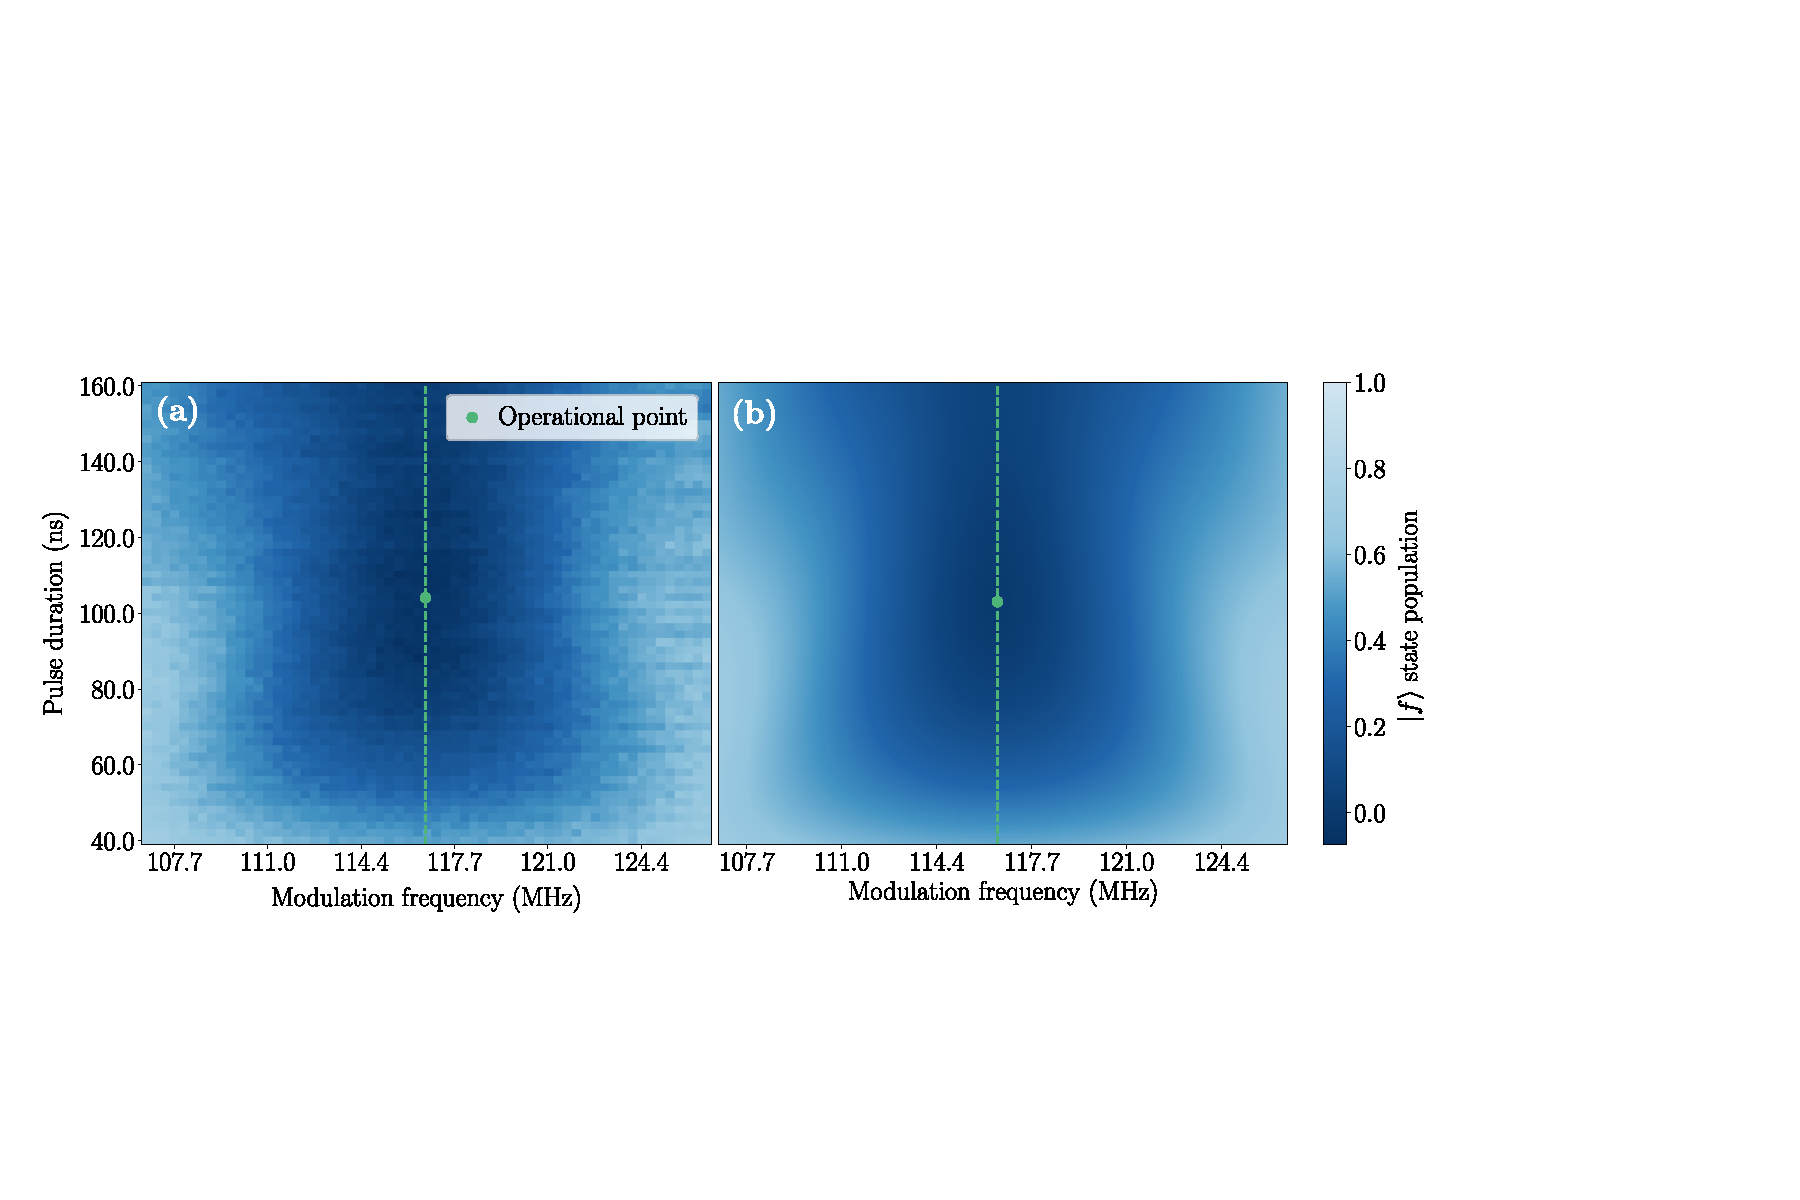
\includegraphics[width = \textwidth]{Images/Chap3/a_2.pdf}
    \caption{\textbf{(a)} data of the $f0e1$ transition within a storage-emitter pair with \textbf{(b)} relative fit}
    \label{fig:CNOT_data}
\end{figure}


\section{Storage-Storage}
\label{sec:S-S}

In the Storage-Storage system (S-S), the extended lifetime of the two qubits allows us to execute single-qubit gates on them.
Additionally, the capability to perform $2\pi$ rotations on the sidebands of this two-qubit system enables the implementation of a CZ gate within the S-S system.

\begin{figure}[b]
    \centering
    

\tikzset{every picture/.style={line width=0.75pt}} %set default line width to 0.75pt        

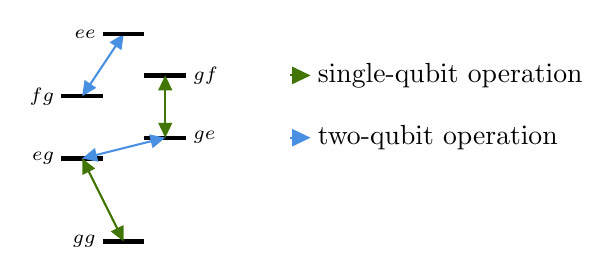
\begin{tikzpicture}[x=0.75pt,y=0.75pt,yscale=-1,xscale=1]
%uncomment if require: \path (0,300); %set diagram left start at 0, and has height of 300

%Straight Lines [id:da9559663622579351] 
\draw [line width=1.5]    (100,100) -- (120,100) ;
%Straight Lines [id:da38130444644691297] 
\draw [line width=1.5]    (140,90) -- (160,90) ;
%Straight Lines [id:da2359488638530448] 
\draw [line width=1.5]    (100,130) -- (120,130) ;
%Straight Lines [id:da3841009239924672] 
\draw [line width=1.5]    (120,170) -- (140,170) ;
%Straight Lines [id:da5788606590900368] 
\draw [line width=1.5]    (140,120) -- (160,120) ;
%Straight Lines [id:da9477773949836692] 
\draw [color={rgb, 255:red, 65; green, 117; blue, 5 }  ,draw opacity=1 ]   (111.34,132.68) -- (128.66,167.32) ;
\draw [shift={(130,170)}, rotate = 243.43] [fill={rgb, 255:red, 65; green, 117; blue, 5 }  ,fill opacity=1 ][line width=0.08]  [draw opacity=0] (7.14,-3.43) -- (0,0) -- (7.14,3.43) -- cycle    ;
\draw [shift={(110,130)}, rotate = 63.43] [fill={rgb, 255:red, 65; green, 117; blue, 5 }  ,fill opacity=1 ][line width=0.08]  [draw opacity=0] (7.14,-3.43) -- (0,0) -- (7.14,3.43) -- cycle    ;
%Straight Lines [id:da6539701699881647] 
\draw [color={rgb, 255:red, 74; green, 144; blue, 226 }  ,draw opacity=1 ]   (128.34,72.5) -- (111.66,97.5) ;
\draw [shift={(110,100)}, rotate = 303.69] [fill={rgb, 255:red, 74; green, 144; blue, 226 }  ,fill opacity=1 ][line width=0.08]  [draw opacity=0] (7.14,-3.43) -- (0,0) -- (7.14,3.43) -- cycle    ;
\draw [shift={(130,70)}, rotate = 123.69] [fill={rgb, 255:red, 74; green, 144; blue, 226 }  ,fill opacity=1 ][line width=0.08]  [draw opacity=0] (7.14,-3.43) -- (0,0) -- (7.14,3.43) -- cycle    ;
%Straight Lines [id:da6430626577491835] 
\draw [color={rgb, 255:red, 65; green, 117; blue, 5 }  ,draw opacity=1 ]   (210,90) -- (217,90) ;
\draw [shift={(220,90)}, rotate = 180] [fill={rgb, 255:red, 65; green, 117; blue, 5 }  ,fill opacity=1 ][line width=0.08]  [draw opacity=0] (8.93,-4.29) -- (0,0) -- (8.93,4.29) -- cycle    ;
%Straight Lines [id:da593444231277527] 
\draw [color={rgb, 255:red, 74; green, 144; blue, 226 }  ,draw opacity=1 ]   (210,120) -- (217,120) ;
\draw [shift={(220,120)}, rotate = 180] [fill={rgb, 255:red, 74; green, 144; blue, 226 }  ,fill opacity=1 ][line width=0.08]  [draw opacity=0] (8.93,-4.29) -- (0,0) -- (8.93,4.29) -- cycle    ;
%Straight Lines [id:da04551771823475548] 
\draw [line width=1.5]    (120,70) -- (140,70) ;
%Straight Lines [id:da8060801042251682] 
\draw [color={rgb, 255:red, 65; green, 117; blue, 5 }  ,draw opacity=1 ]   (150,93) -- (150,117) ;
\draw [shift={(150,120)}, rotate = 270] [fill={rgb, 255:red, 65; green, 117; blue, 5 }  ,fill opacity=1 ][line width=0.08]  [draw opacity=0] (7.14,-3.43) -- (0,0) -- (7.14,3.43) -- cycle    ;
\draw [shift={(150,90)}, rotate = 90] [fill={rgb, 255:red, 65; green, 117; blue, 5 }  ,fill opacity=1 ][line width=0.08]  [draw opacity=0] (7.14,-3.43) -- (0,0) -- (7.14,3.43) -- cycle    ;
%Straight Lines [id:da40683969551339827] 
\draw [color={rgb, 255:red, 74; green, 144; blue, 226 }  ,draw opacity=1 ]   (112.91,129.27) -- (147.09,120.73) ;
\draw [shift={(150,120)}, rotate = 165.96] [fill={rgb, 255:red, 74; green, 144; blue, 226 }  ,fill opacity=1 ][line width=0.08]  [draw opacity=0] (7.14,-3.43) -- (0,0) -- (7.14,3.43) -- cycle    ;
\draw [shift={(110,130)}, rotate = 345.96] [fill={rgb, 255:red, 74; green, 144; blue, 226 }  ,fill opacity=1 ][line width=0.08]  [draw opacity=0] (7.14,-3.43) -- (0,0) -- (7.14,3.43) -- cycle    ;

% Text Node
\draw (98,100) node [anchor=east] [inner sep=0.75pt]  [font=\scriptsize]  {$fg$};
% Text Node
\draw (98,130) node [anchor=east] [inner sep=0.75pt]  [font=\scriptsize]  {$eg$};
% Text Node
\draw (118,170) node [anchor=east] [inner sep=0.75pt]  [font=\scriptsize]  {$gg$};
% Text Node
\draw (162,90) node [anchor=west] [inner sep=0.75pt]  [font=\scriptsize]  {$gf$};
% Text Node
\draw (162,120) node [anchor=west] [inner sep=0.75pt]  [font=\scriptsize]  {$ge$};
% Text Node
\draw (222,90) node [anchor=west] [inner sep=0.75pt]   [align=left] {single-qubit operation};
% Text Node
\draw (222,120) node [anchor=west] [inner sep=0.75pt]   [align=left] {two-qubit operation};
% Text Node
\draw (118,70) node [anchor=east] [inner sep=0.75pt]  [font=\scriptsize]  {$ee$};


\end{tikzpicture}
    \vspace{-1cm}
    \caption{Level diagram of storage-storage interaction}
    \label{fig:SS_level}
\end{figure}

In \cref{fig:SS_level}, the energy levels of the two-qubits system is shown, together with some single- and two-qubit gates that we can run on them.

\subsection{CZ}

The unitary matrix representing a controlled-phase gate, or CZ, is
\begin{equation}
    U_{\text{CZ}} = 
    \begin{pmatrix}
    1 & 0 & 0 & 0 \\
    0 & 1 & 0 & 0 \\
    0 & 0 & 1 & 0 \\
    0 & 0 & 0 & -1 \\
\end{pmatrix}.
\end{equation}

It performs the operation
\begin{equation}
    (\alpha \ket{gg} + \beta \ket{ge} + \gamma \ket{eg} + \delta \ket{ee})_{\text{S}_1 \text{S}_2} \xrightarrow{U_{\text{CZ}}}
    (\alpha \ket{gg} + \beta \ket{ge} + \gamma \ket{eg} - \delta \ket{ee})_{\text{S}_1 \text{S}_2} . 
\end{equation}

The operational sequence on our device involves transferring population between the states $\ket{ee}$ and $\ket{fg}$ within the S-S system.
After a $2\pi$ rotation, the population returns to the $\ket{ee}$ state, but with an opposite phase (see \cref{fig:SS_CZ}), effectively implementing a CZ gate.

\begin{figure}
    \centering
    

\tikzset{every picture/.style={line width=0.75pt}} %set default line width to 0.75pt        

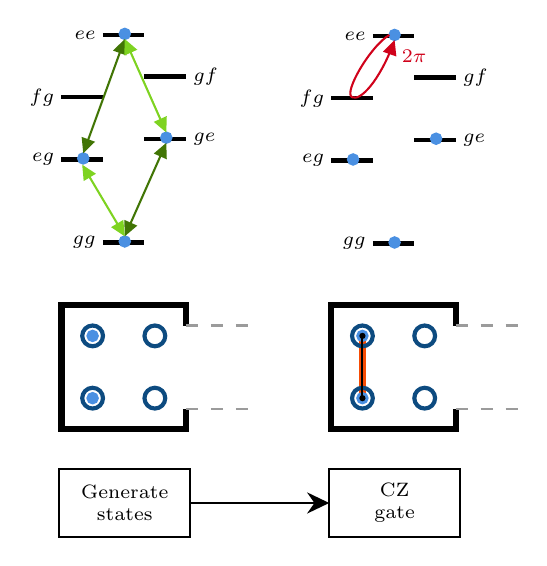
\begin{tikzpicture}[x=0.75pt,y=0.75pt,yscale=-1,xscale=1]
%uncomment if require: \path (0,369); %set diagram left start at 0, and has height of 369

%Straight Lines [id:da14238319538466393] 
\draw [color={rgb, 255:red, 246; green, 76; blue, 4 }  ,draw opacity=1 ][line width=2.25]    (185,215) -- (185,245) ;
%Shape: Circle [id:dp6131452055369363] 
\draw  [color={rgb, 255:red, 13; green, 75; blue, 128 }  ,draw opacity=1 ][line width=1.5]  (180,215) .. controls (180,212.24) and (182.24,210) .. (185,210) .. controls (187.76,210) and (190,212.24) .. (190,215) .. controls (190,217.76) and (187.76,220) .. (185,220) .. controls (182.24,220) and (180,217.76) .. (180,215) -- cycle ;
%Shape: Circle [id:dp044196496820445685] 
\draw  [color={rgb, 255:red, 13; green, 75; blue, 128 }  ,draw opacity=1 ][line width=1.5]  (180,245) .. controls (180,242.24) and (182.24,240) .. (185,240) .. controls (187.76,240) and (190,242.24) .. (190,245) .. controls (190,247.76) and (187.76,250) .. (185,250) .. controls (182.24,250) and (180,247.76) .. (180,245) -- cycle ;
%Shape: Circle [id:dp5885154746260259] 
\draw  [color={rgb, 255:red, 13; green, 75; blue, 128 }  ,draw opacity=1 ][line width=1.5]  (210,245) .. controls (210,242.24) and (212.24,240) .. (215,240) .. controls (217.76,240) and (220,242.24) .. (220,245) .. controls (220,247.76) and (217.76,250) .. (215,250) .. controls (212.24,250) and (210,247.76) .. (210,245) -- cycle ;
%Shape: Circle [id:dp7469388514126467] 
\draw  [color={rgb, 255:red, 13; green, 75; blue, 128 }  ,draw opacity=1 ][line width=1.5]  (210,215) .. controls (210,212.24) and (212.24,210) .. (215,210) .. controls (217.76,210) and (220,212.24) .. (220,215) .. controls (220,217.76) and (217.76,220) .. (215,220) .. controls (212.24,220) and (210,217.76) .. (210,215) -- cycle ;
%Shape: Square [id:dp8509793592974496] 
\draw  [line width=2.25]  (170,200) -- (230,200) -- (230,260) -- (170,260) -- cycle ;
%Straight Lines [id:da12483962352096123] 
\draw [color={rgb, 255:red, 255; green, 255; blue, 255 }  ,draw opacity=1 ][line width=3]    (230,210) -- (230,250) ;

%Shape: Circle [id:dp2946136793659927] 
\draw  [color={rgb, 255:red, 74; green, 144; blue, 226 }  ,draw opacity=1 ][fill={rgb, 255:red, 74; green, 144; blue, 226 }  ,fill opacity=1 ] (182.5,215) .. controls (182.5,213.62) and (183.62,212.5) .. (185,212.5) .. controls (186.38,212.5) and (187.5,213.62) .. (187.5,215) .. controls (187.5,216.38) and (186.38,217.5) .. (185,217.5) .. controls (183.62,217.5) and (182.5,216.38) .. (182.5,215) -- cycle ;
%Straight Lines [id:da5174133920036248] 
\draw [color={rgb, 255:red, 155; green, 155; blue, 155 }  ,draw opacity=1 ] [dash pattern={on 4.5pt off 4.5pt}]  (230,210) -- (260,210) ;
%Straight Lines [id:da26746057224200814] 
\draw [color={rgb, 255:red, 155; green, 155; blue, 155 }  ,draw opacity=1 ] [dash pattern={on 4.5pt off 4.5pt}]  (230,250) -- (260,250) ;
%Shape: Circle [id:dp9726522957124347] 
\draw  [color={rgb, 255:red, 13; green, 75; blue, 128 }  ,draw opacity=1 ][line width=1.5]  (50,215) .. controls (50,212.24) and (52.24,210) .. (55,210) .. controls (57.76,210) and (60,212.24) .. (60,215) .. controls (60,217.76) and (57.76,220) .. (55,220) .. controls (52.24,220) and (50,217.76) .. (50,215) -- cycle ;
%Shape: Circle [id:dp5051693054900083] 
\draw  [color={rgb, 255:red, 13; green, 75; blue, 128 }  ,draw opacity=1 ][line width=1.5]  (50,245) .. controls (50,242.24) and (52.24,240) .. (55,240) .. controls (57.76,240) and (60,242.24) .. (60,245) .. controls (60,247.76) and (57.76,250) .. (55,250) .. controls (52.24,250) and (50,247.76) .. (50,245) -- cycle ;
%Shape: Circle [id:dp6033756962982088] 
\draw  [color={rgb, 255:red, 13; green, 75; blue, 128 }  ,draw opacity=1 ][line width=1.5]  (80,245) .. controls (80,242.24) and (82.24,240) .. (85,240) .. controls (87.76,240) and (90,242.24) .. (90,245) .. controls (90,247.76) and (87.76,250) .. (85,250) .. controls (82.24,250) and (80,247.76) .. (80,245) -- cycle ;
%Shape: Circle [id:dp651180579558279] 
\draw  [color={rgb, 255:red, 13; green, 75; blue, 128 }  ,draw opacity=1 ][line width=1.5]  (80,215) .. controls (80,212.24) and (82.24,210) .. (85,210) .. controls (87.76,210) and (90,212.24) .. (90,215) .. controls (90,217.76) and (87.76,220) .. (85,220) .. controls (82.24,220) and (80,217.76) .. (80,215) -- cycle ;
%Shape: Square [id:dp8220576054517261] 
\draw  [line width=2.25]  (40,200) -- (100,200) -- (100,260) -- (40,260) -- cycle ;
%Straight Lines [id:da3250679662921139] 
\draw [color={rgb, 255:red, 255; green, 255; blue, 255 }  ,draw opacity=1 ][line width=3]    (100,210) -- (100,250) ;

%Shape: Circle [id:dp1764454757841779] 
\draw  [color={rgb, 255:red, 74; green, 144; blue, 226 }  ,draw opacity=1 ][fill={rgb, 255:red, 74; green, 144; blue, 226 }  ,fill opacity=1 ] (52.5,215) .. controls (52.5,213.62) and (53.62,212.5) .. (55,212.5) .. controls (56.38,212.5) and (57.5,213.62) .. (57.5,215) .. controls (57.5,216.38) and (56.38,217.5) .. (55,217.5) .. controls (53.62,217.5) and (52.5,216.38) .. (52.5,215) -- cycle ;
%Straight Lines [id:da9570390374106923] 
\draw [color={rgb, 255:red, 155; green, 155; blue, 155 }  ,draw opacity=1 ] [dash pattern={on 4.5pt off 4.5pt}]  (100,210) -- (130,210) ;
%Straight Lines [id:da8355397813605424] 
\draw [color={rgb, 255:red, 155; green, 155; blue, 155 }  ,draw opacity=1 ] [dash pattern={on 4.5pt off 4.5pt}]  (100,250) -- (130,250) ;
%Straight Lines [id:da605984992083237] 
\draw [line width=1.5]    (40,100) -- (60,100) ;
%Straight Lines [id:da38731851189389244] 
\draw [line width=1.5]    (80,90) -- (100,90) ;
%Straight Lines [id:da4898165874704924] 
\draw [line width=1.5]    (40,130) -- (60,130) ;
%Straight Lines [id:da24826706546268984] 
\draw [line width=1.5]    (60,170) -- (80,170) ;
%Straight Lines [id:da43859897810303505] 
\draw [line width=1.5]    (80,120) -- (100,120) ;
%Straight Lines [id:da33344037757379863] 
\draw [line width=1.5]    (60,70) -- (80,70) ;
%Shape: Circle [id:dp7629931524746876] 
\draw  [color={rgb, 255:red, 74; green, 144; blue, 226 }  ,draw opacity=1 ][fill={rgb, 255:red, 74; green, 144; blue, 226 }  ,fill opacity=1 ] (68,169.5) .. controls (68,168.12) and (69.12,167) .. (70.5,167) .. controls (71.88,167) and (73,168.12) .. (73,169.5) .. controls (73,170.88) and (71.88,172) .. (70.5,172) .. controls (69.12,172) and (68,170.88) .. (68,169.5) -- cycle ;
%Shape: Circle [id:dp9222004689061901] 
\draw  [color={rgb, 255:red, 74; green, 144; blue, 226 }  ,draw opacity=1 ][fill={rgb, 255:red, 74; green, 144; blue, 226 }  ,fill opacity=1 ] (48,129.5) .. controls (48,128.12) and (49.12,127) .. (50.5,127) .. controls (51.88,127) and (53,128.12) .. (53,129.5) .. controls (53,130.88) and (51.88,132) .. (50.5,132) .. controls (49.12,132) and (48,130.88) .. (48,129.5) -- cycle ;
%Shape: Circle [id:dp5632081381008429] 
\draw  [color={rgb, 255:red, 74; green, 144; blue, 226 }  ,draw opacity=1 ][fill={rgb, 255:red, 74; green, 144; blue, 226 }  ,fill opacity=1 ] (88,119.5) .. controls (88,118.12) and (89.12,117) .. (90.5,117) .. controls (91.88,117) and (93,118.12) .. (93,119.5) .. controls (93,120.88) and (91.88,122) .. (90.5,122) .. controls (89.12,122) and (88,120.88) .. (88,119.5) -- cycle ;
%Shape: Circle [id:dp023555240322724158] 
\draw  [color={rgb, 255:red, 74; green, 144; blue, 226 }  ,draw opacity=1 ][fill={rgb, 255:red, 74; green, 144; blue, 226 }  ,fill opacity=1 ] (68,69.5) .. controls (68,68.12) and (69.12,67) .. (70.5,67) .. controls (71.88,67) and (73,68.12) .. (73,69.5) .. controls (73,70.88) and (71.88,72) .. (70.5,72) .. controls (69.12,72) and (68,70.88) .. (68,69.5) -- cycle ;
%Straight Lines [id:da4406201929591368] 
\draw [color={rgb, 255:red, 65; green, 117; blue, 5 }  ,draw opacity=1 ]   (89.28,124.74) -- (71.72,164.26) ;
\draw [shift={(70.5,167)}, rotate = 293.96] [fill={rgb, 255:red, 65; green, 117; blue, 5 }  ,fill opacity=1 ][line width=0.08]  [draw opacity=0] (7.14,-3.43) -- (0,0) -- (7.14,3.43) -- cycle    ;
\draw [shift={(90.5,122)}, rotate = 113.96] [fill={rgb, 255:red, 65; green, 117; blue, 5 }  ,fill opacity=1 ][line width=0.08]  [draw opacity=0] (7.14,-3.43) -- (0,0) -- (7.14,3.43) -- cycle    ;
%Straight Lines [id:da9819884495181663] 
\draw [color={rgb, 255:red, 65; green, 117; blue, 5 }  ,draw opacity=1 ]   (69.47,74.82) -- (51.53,124.18) ;
\draw [shift={(50.5,127)}, rotate = 289.98] [fill={rgb, 255:red, 65; green, 117; blue, 5 }  ,fill opacity=1 ][line width=0.08]  [draw opacity=0] (7.14,-3.43) -- (0,0) -- (7.14,3.43) -- cycle    ;
\draw [shift={(70.5,72)}, rotate = 109.98] [fill={rgb, 255:red, 65; green, 117; blue, 5 }  ,fill opacity=1 ][line width=0.08]  [draw opacity=0] (7.14,-3.43) -- (0,0) -- (7.14,3.43) -- cycle    ;
%Straight Lines [id:da9796916063314295] 
\draw [color={rgb, 255:red, 126; green, 211; blue, 33 }  ,draw opacity=1 ]   (71.72,74.74) -- (89.28,114.26) ;
\draw [shift={(90.5,117)}, rotate = 246.04] [fill={rgb, 255:red, 126; green, 211; blue, 33 }  ,fill opacity=1 ][line width=0.08]  [draw opacity=0] (7.14,-3.43) -- (0,0) -- (7.14,3.43) -- cycle    ;
\draw [shift={(70.5,72)}, rotate = 66.04] [fill={rgb, 255:red, 126; green, 211; blue, 33 }  ,fill opacity=1 ][line width=0.08]  [draw opacity=0] (7.14,-3.43) -- (0,0) -- (7.14,3.43) -- cycle    ;
%Straight Lines [id:da25683659760281263] 
\draw [color={rgb, 255:red, 126; green, 211; blue, 33 }  ,draw opacity=1 ]   (51.53,135.08) -- (68.97,164.42) ;
\draw [shift={(70.5,167)}, rotate = 239.28] [fill={rgb, 255:red, 126; green, 211; blue, 33 }  ,fill opacity=1 ][line width=0.08]  [draw opacity=0] (7.14,-3.43) -- (0,0) -- (7.14,3.43) -- cycle    ;
\draw [shift={(50,132.5)}, rotate = 59.28] [fill={rgb, 255:red, 126; green, 211; blue, 33 }  ,fill opacity=1 ][line width=0.08]  [draw opacity=0] (7.14,-3.43) -- (0,0) -- (7.14,3.43) -- cycle    ;
%Straight Lines [id:da9637012758897168] 
\draw [line width=1.5]    (170,100.5) -- (190,100.5) ;
%Straight Lines [id:da8684535686248622] 
\draw [line width=1.5]    (210,90.5) -- (230,90.5) ;
%Straight Lines [id:da17021177110230912] 
\draw [line width=1.5]    (170,130.5) -- (190,130.5) ;
%Straight Lines [id:da7796352034758786] 
\draw [line width=1.5]    (190,170.5) -- (210,170.5) ;
%Straight Lines [id:da41159550798158584] 
\draw [line width=1.5]    (210,120.5) -- (230,120.5) ;
%Straight Lines [id:da7308144564661493] 
\draw [line width=1.5]    (190,70.5) -- (210,70.5) ;
%Shape: Circle [id:dp8827634585194027] 
\draw  [color={rgb, 255:red, 74; green, 144; blue, 226 }  ,draw opacity=1 ][fill={rgb, 255:red, 74; green, 144; blue, 226 }  ,fill opacity=1 ] (198,170) .. controls (198,168.62) and (199.12,167.5) .. (200.5,167.5) .. controls (201.88,167.5) and (203,168.62) .. (203,170) .. controls (203,171.38) and (201.88,172.5) .. (200.5,172.5) .. controls (199.12,172.5) and (198,171.38) .. (198,170) -- cycle ;
%Shape: Circle [id:dp12686587985832598] 
\draw  [color={rgb, 255:red, 74; green, 144; blue, 226 }  ,draw opacity=1 ][fill={rgb, 255:red, 74; green, 144; blue, 226 }  ,fill opacity=1 ] (178,130) .. controls (178,128.62) and (179.12,127.5) .. (180.5,127.5) .. controls (181.88,127.5) and (183,128.62) .. (183,130) .. controls (183,131.38) and (181.88,132.5) .. (180.5,132.5) .. controls (179.12,132.5) and (178,131.38) .. (178,130) -- cycle ;
%Shape: Circle [id:dp6893004504301061] 
\draw  [color={rgb, 255:red, 74; green, 144; blue, 226 }  ,draw opacity=1 ][fill={rgb, 255:red, 74; green, 144; blue, 226 }  ,fill opacity=1 ] (218,120) .. controls (218,118.62) and (219.12,117.5) .. (220.5,117.5) .. controls (221.88,117.5) and (223,118.62) .. (223,120) .. controls (223,121.38) and (221.88,122.5) .. (220.5,122.5) .. controls (219.12,122.5) and (218,121.38) .. (218,120) -- cycle ;
%Shape: Circle [id:dp6629315947880386] 
\draw  [color={rgb, 255:red, 74; green, 144; blue, 226 }  ,draw opacity=1 ][fill={rgb, 255:red, 74; green, 144; blue, 226 }  ,fill opacity=1 ] (198,70) .. controls (198,68.62) and (199.12,67.5) .. (200.5,67.5) .. controls (201.88,67.5) and (203,68.62) .. (203,70) .. controls (203,71.38) and (201.88,72.5) .. (200.5,72.5) .. controls (199.12,72.5) and (198,71.38) .. (198,70) -- cycle ;
%Curve Lines [id:da5178021924441131] 
\draw [color={rgb, 255:red, 208; green, 2; blue, 27 }  ,draw opacity=1 ]   (198,70) .. controls (189,75.17) and (175.67,97.83) .. (180,100) .. controls (184.12,102.06) and (193.05,91.93) .. (199.5,75.2) ;
\draw [shift={(200.5,72.5)}, rotate = 109.52] [fill={rgb, 255:red, 208; green, 2; blue, 27 }  ,fill opacity=1 ][line width=0.08]  [draw opacity=0] (7.14,-3.43) -- (0,0) -- (7.14,3.43) -- cycle    ;
%Shape: Circle [id:dp26197554740985884] 
\draw  [color={rgb, 255:red, 74; green, 144; blue, 226 }  ,draw opacity=1 ][fill={rgb, 255:red, 74; green, 144; blue, 226 }  ,fill opacity=1 ] (52.5,245) .. controls (52.5,243.62) and (53.62,242.5) .. (55,242.5) .. controls (56.38,242.5) and (57.5,243.62) .. (57.5,245) .. controls (57.5,246.38) and (56.38,247.5) .. (55,247.5) .. controls (53.62,247.5) and (52.5,246.38) .. (52.5,245) -- cycle ;
%Shape: Circle [id:dp7779633747567205] 
\draw  [color={rgb, 255:red, 74; green, 144; blue, 226 }  ,draw opacity=1 ][fill={rgb, 255:red, 74; green, 144; blue, 226 }  ,fill opacity=1 ] (182.5,245) .. controls (182.5,243.62) and (183.62,242.5) .. (185,242.5) .. controls (186.38,242.5) and (187.5,243.62) .. (187.5,245) .. controls (187.5,246.38) and (186.38,247.5) .. (185,247.5) .. controls (183.62,247.5) and (182.5,246.38) .. (182.5,245) -- cycle ;
%Straight Lines [id:da5417689626607565] 
\draw    (185,215) -- (185,245) ;
%Shape: Circle [id:dp8939955847994656] 
\draw  [draw opacity=0][fill={rgb, 255:red, 0; green, 0; blue, 0 }  ,fill opacity=1 ] (183.5,215) .. controls (183.5,214.17) and (184.17,213.5) .. (185,213.5) .. controls (185.83,213.5) and (186.5,214.17) .. (186.5,215) .. controls (186.5,215.83) and (185.83,216.5) .. (185,216.5) .. controls (184.17,216.5) and (183.5,215.83) .. (183.5,215) -- cycle ;
%Shape: Circle [id:dp5788101040789697] 
\draw  [draw opacity=0][fill={rgb, 255:red, 0; green, 0; blue, 0 }  ,fill opacity=1 ] (183.5,245) .. controls (183.5,244.17) and (184.17,243.5) .. (185,243.5) .. controls (185.83,243.5) and (186.5,244.17) .. (186.5,245) .. controls (186.5,245.83) and (185.83,246.5) .. (185,246.5) .. controls (184.17,246.5) and (183.5,245.83) .. (183.5,245) -- cycle ;

% Text Node
\draw (202.5,75.9) node [anchor=north west][inner sep=0.75pt]  [font=\scriptsize,color={rgb, 255:red, 208; green, 2; blue, 27 }  ,opacity=1 ]  {$2\pi $};
% Text Node
\draw    (169,279) -- (232,279) -- (232,312) -- (169,312) -- cycle  ;
\draw (200.5,295.5) node  [font=\scriptsize] [align=left] {\begin{minipage}[lt]{40.8pt}\setlength\topsep{0pt}
\begin{center}
CZ\\gate
\end{center}

\end{minipage}};
% Text Node
\draw    (39,279) -- (102,279) -- (102,312) -- (39,312) -- cycle  ;
\draw (70.5,295.5) node  [font=\scriptsize] [align=left] {\begin{minipage}[lt]{40.8pt}\setlength\topsep{0pt}
\begin{center}
Generate\\states
\end{center}

\end{minipage}};
% Text Node
\draw (38,100) node [anchor=east] [inner sep=0.75pt]  [font=\scriptsize]  {$fg$};
% Text Node
\draw (38,130) node [anchor=east] [inner sep=0.75pt]  [font=\scriptsize]  {$eg$};
% Text Node
\draw (58,170) node [anchor=east] [inner sep=0.75pt]  [font=\scriptsize]  {$gg$};
% Text Node
\draw (102,90) node [anchor=west] [inner sep=0.75pt]  [font=\scriptsize]  {$gf$};
% Text Node
\draw (102,120) node [anchor=west] [inner sep=0.75pt]  [font=\scriptsize]  {$ge$};
% Text Node
\draw (58,70) node [anchor=east] [inner sep=0.75pt]  [font=\scriptsize]  {$ee$};
% Text Node
\draw (168,100.5) node [anchor=east] [inner sep=0.75pt]  [font=\scriptsize]  {$fg$};
% Text Node
\draw (168,130.5) node [anchor=east] [inner sep=0.75pt]  [font=\scriptsize]  {$eg$};
% Text Node
\draw (188,170.5) node [anchor=east] [inner sep=0.75pt]  [font=\scriptsize]  {$gg$};
% Text Node
\draw (232,90.5) node [anchor=west] [inner sep=0.75pt]  [font=\scriptsize]  {$gf$};
% Text Node
\draw (232,120.5) node [anchor=west] [inner sep=0.75pt]  [font=\scriptsize]  {$ge$};
% Text Node
\draw (188,70.5) node [anchor=east] [inner sep=0.75pt]  [font=\scriptsize]  {$ee$};
% Connection
\draw    (102,295.5) -- (166,295.5) ;
\draw [shift={(169,295.5)}, rotate = 180] [fill={rgb, 255:red, 0; green, 0; blue, 0 }  ][line width=0.08]  [draw opacity=0] (10.72,-5.15) -- (0,0) -- (10.72,5.15) -- (7.12,0) -- cycle    ;

\end{tikzpicture}
    \vspace{-1cm}
    \caption{Protocol for S-S CZ gate}
    \label{fig:SS_CZ}
\end{figure}

In this context, it is necessary to calibrate the interaction between the $ee$ and $fg$ energy levels.
For this purpose, we employ the previously derived model, using \cref{eq:chevron} to perform fitting on the data.
Fig.~\ref{fig:Chev_data} shows the data and the respective fit.
It also shows the operational point for implementing the CZ gate.
This operational point is given by
\begin{equation}
    \widetilde{t} = \frac{1}{2 g_0}.
\end{equation}

\begin{figure}
    \centering
    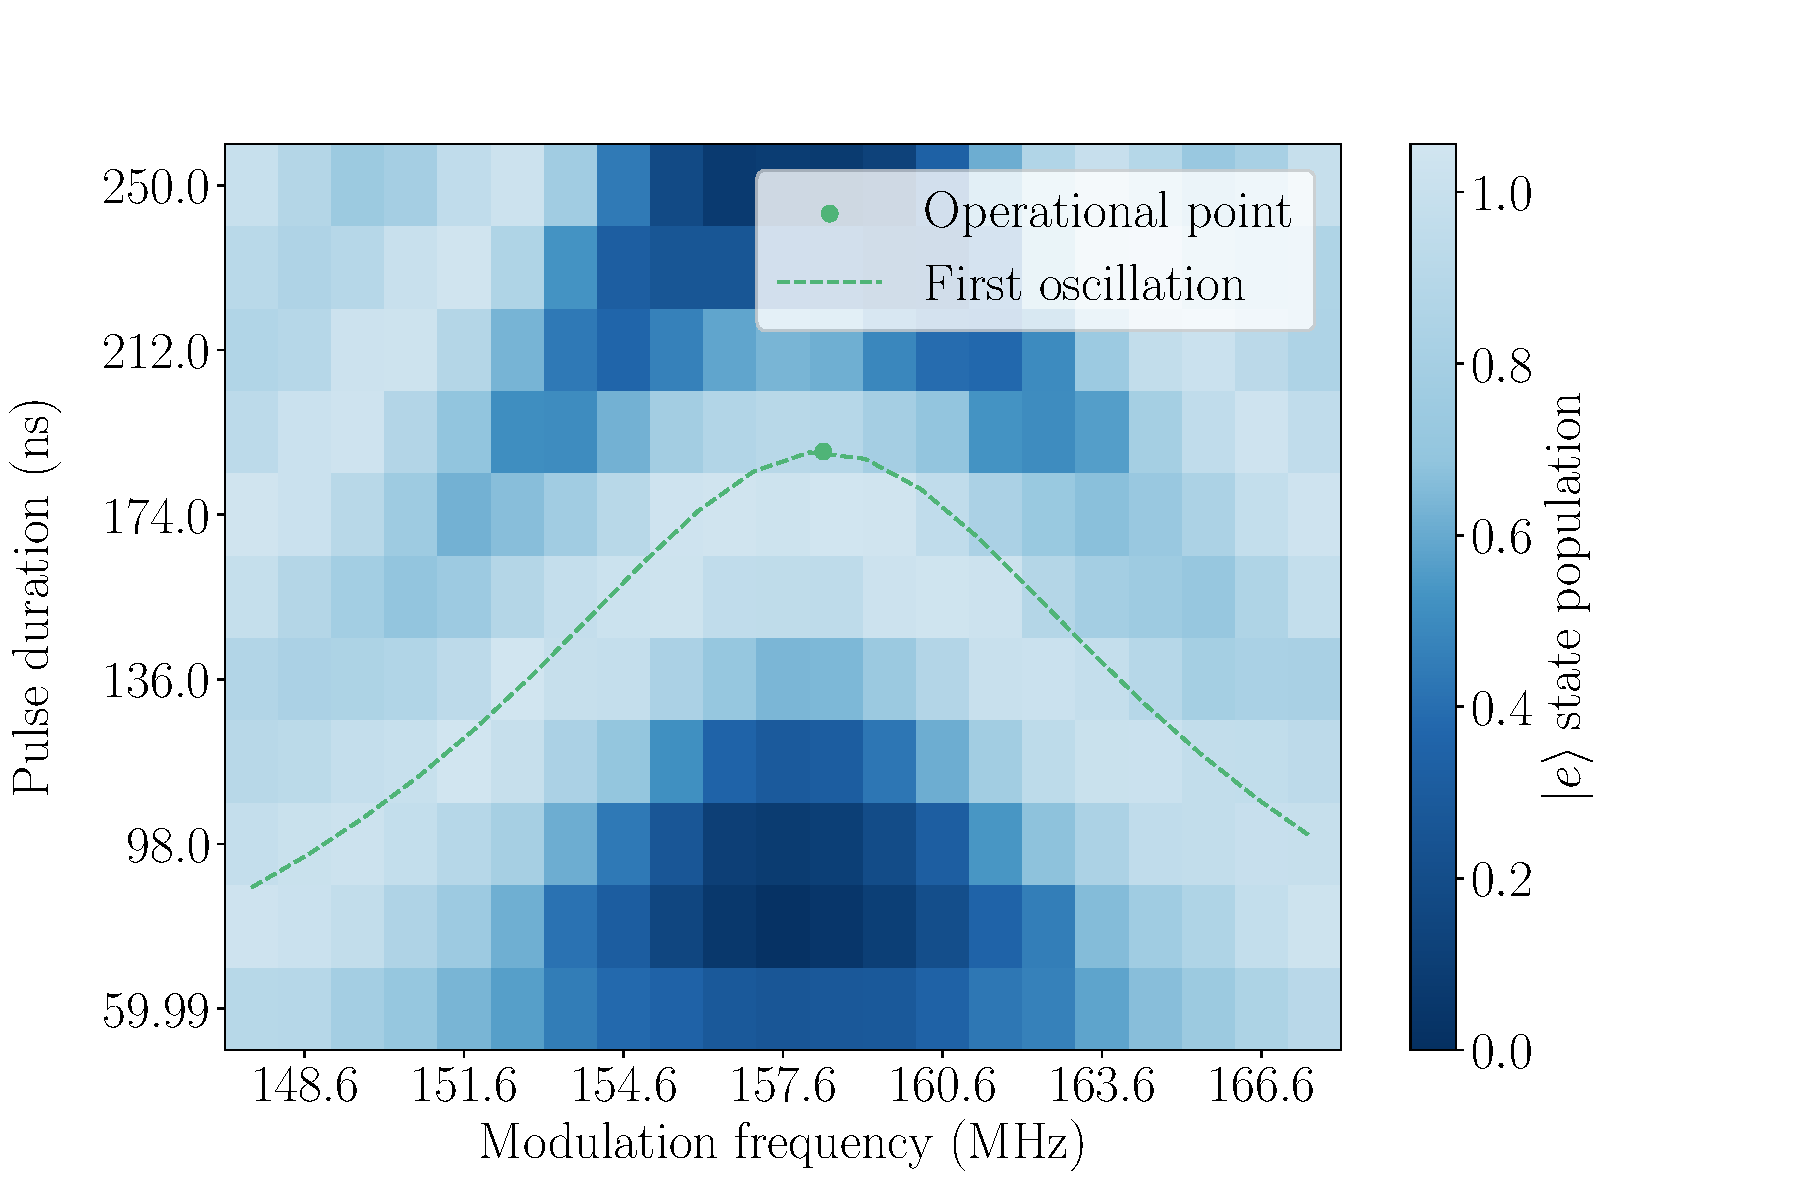
\includegraphics[width=0.8\linewidth]{Images//Chap3/Chevron_data.pdf}
    \caption{Data of the $eefg$ sideband transition between the two storage qubits}
    \label{fig:Chev_data}
\end{figure}

On \cref{fig:Chev_data} is also depicted the first oscillation period as a function of the detuning $\delta$, given by
\begin{equation}
    t = \frac{1}{\sqrt{4 g_0^2 + \delta^2}} . 
\end{equation}